f\documentclass{article}

\usepackage{fullpage}
\usepackage{lineno}
\usepackage{wrapfig}
\usepackage{graphicx,color}
\usepackage{amssymb}
\usepackage{subcaption}
\usepackage{braket}
\usepackage{physics}
\usepackage{yquant}
\usepackage{tikz}
\usetikzlibrary{quantikz,fit,svg.path}
\usepackage[backend=biber,citestyle=numeric-comp]{biblatex}
\addbibresource{cites.bib}
\ExecuteBibliographyOptions{sorting=nyt,maxbibnames=100,doi=false,isbn=false,url=false}

\newcommand{\x}{\textsc{x}}
\newcommand{\cx}{\textsc{cx}}
\newcommand{\ccx}{\textsc{ccx}}
\newcommand{\cccx}{\textsc{cccx}}
\newcommand{\qket}[1]{\ket{\tilde{#1}}}
\newcommand{\preim}[2]{\{\cdot\stackrel{#1}{\longleftarrow}{#2}\}}
\newcommand{\finset}[1]{[\mathbf{#1}]}
\newcommand{\red}[1]{{\color{red}{#1}}}
\newcommand{\todo}[1]{\fbox{\begin{minipage}{25em}{\red{#1}}\end{minipage}}}

\linenumbers

%%%%%%%%%%%%%%%%%%%%%%%%%%%%%%%%%%%%%%%%%%%%%%%%%%%%%%%%%%%%%%%%%%%%%%%%%%%%%%%%%%%%%%%%%%
\title{De-Quantizing Quantum Algorithms by Retrodictive Execution}
\author{Jacques Carette \qquad Gerardo Ortiz$^{*}$ \qquad Amr Sabry \\
McMaster University \qquad Indiana University \qquad Indiana University}
\begin{document}
\maketitle

%% 200 words

\begin{abstract}
  just run forward symbolically
  retrodictive is not fundamental here
  
  
The quantum circuit model consists of two classes of gates: (i)
quantum counterparts to classical reversible gates (e.g., Toffoli
gates), and (ii) genuine quantum gates with no classical counterpart
(e.g., Hadamard and phase gates). We make the remarkable observation,
that, for a number of well-established quantum algorithms, judicious
reasoning about the classical components, ignoring all the quantum
gates, is sufficient. Put differently, in those cases, the quantum
gates serve no fundamental purpose and are actually distracting from
an underlying efficient classical algorithm. The result relies on the
ability to symbolically execute circuits, especially in a retrodictive
fashion, i.e., by making partial observations at the output site and
proceeding backwards to infer the implied initial conditions.
\end{abstract}

%%%%%%%%%%%%%%%%%%%%%%%%%%%%%%%%%%%%%%%%%%%%%%%%%%%%%%%%%%%%%%%%%%%%%%%%%%%%%%%%%%%%%%%%%%
\section{Main}
\begin{refsection}
%% main text 2500 - 4300 words
%% 5-6 figures

\begin{quote}
You can’t connect the dots looking forward; you can only connect them
looking backwards.  So you have to trust that the dots will somehow
connect in your future. \emph{Steve Jobs}
\end{quote}

%% \begin{wrapfigure}{r}{5cm}
%% \begin{quantikz}[row sep=0.7cm,column sep=1cm]
%%    \qw & 
%%    \gate[wires=2][2.5cm]{U_f}\gateinput{$x$}\gateoutput{$x$} &
%%    \qw
%%    \\
%%    \qw &
%%    \gateinput{$y$}\gateoutput{$f(x)\oplus y$} &
%%    \qw
%% \end{quantikz}
%% \caption{\label{fig:oracle}Quantum oracle}
%% \end{wrapfigure}

%% \begin{wrapfigure}{r}{6cm}
%% \begin{tikzpicture}[scale=1]
%%     \begin{yquant*}[register/minimum height=1.3cm]
%%     qubit {$x$} x;
%%     qubit {$\ket{0}$} y;
%%     hspace {5mm} -;
%%     [x radius=1.3cm]
%%     box {$U_f$} (x,y);
%%     hspace {5mm} -;
%%     output {$x$} x;
%%     measure y; 
%%   \end{yquant*}
%%   \draw[line width=3pt, ->, blue] (3.5,-2.1) .. controls (-0.2,-1.6) and (-0.2,-1.1) .. (3.5,-0.6);
%% \end{tikzpicture}
%% \caption{\label{fig:flow}Retrodictive execution flow}
%% \end{wrapfigure}

Retrodictive quantum theory~\cite{sym13040586},
retrocausality~\cite{Aharonov2008}, and the time-symmetry of physical
laws~\cite{RevModPhys.27.179} suggest that partial knowledge about the
future can be exploited to understand the present. We demonstrate the
even stronger proposition that, in concert with the computational
concepts of \emph{demand-driven lazy evaluation}~\cite{lazyevaluator}
and \emph{symbolic partial evaluation}~\cite{futamura}, retrodictive
reasoning can be used as a computational resource to de-quantize some
quantum algorithms, i.e., to provide efficient classical algorithms
inspired by their quantum counterparts.

\begin{figure}[ht]
  \begin{subfigure}{0.5\textwidth}
  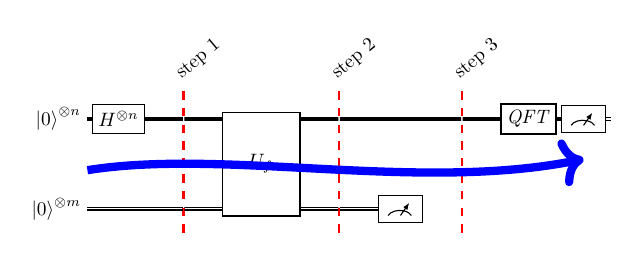
\begin{tikzpicture}[scale=0.7,every label/.style={rotate=40, anchor=south west}]
    \begin{yquant*}[operators/every barrier/.append style={red, thick},
        operator/minimum width=7mm,
        operator/separation=1mm,
        register/separation=10mm]
    qubits {$\ket0^{\otimes n}$} a;
    qubits {$\ket0^{\otimes m}$} b;
    box {$H^{\otimes n}$} a;
    ["step 1"]
    barrier (-);
    [x radius=7mm]
    box {$U_f$} (a,b);
    ["step 2"]
    barrier (-);
    measure b;
    discard b;
    ["step 3"]
    barrier (-);
    box {$\mathit{QFT}$} a;
    measure a;
    \end{yquant*}
    \draw[line width=3pt, ->, blue] (0,-1.2) .. controls (2.5,-0.8) and (6,-1.6) .. (9,-1);
  \end{tikzpicture}
  \caption{Conventional Flow}
  \end{subfigure}
  \begin{subfigure}{0.5\textwidth}
  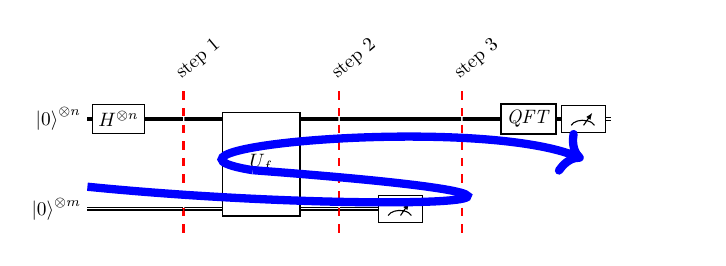
\begin{tikzpicture}[scale=0.7,every label/.style={rotate=40, anchor=south west}]
    \begin{yquant*}[operators/every barrier/.append style={red, thick},
        operator/minimum width=7mm,
        operator/separation=1mm,
        register/separation=10mm]
    qubits {$\ket0^{\otimes n}$} a;
    qubits {$\ket0^{\otimes m}$} b;
    box {$H^{\otimes n}$} a;
    ["step 1"]
    barrier (-);
    [x radius=7mm]
    box {$U_f$} (a,b);
    ["step 2"]
    barrier (-);
    measure b;
    discard b;
    ["step 3"]
    barrier (-);
    box {$\mathit{QFT}$} a;
    measure a;
  \end{yquant*}
  \draw[line width=3pt, blue] (0,-1.5) .. controls (5,-2) and (11,-1.8) .. (3,-1.2);
  \draw[line width=3pt, ->, blue] (3,-1.2) .. controls (0.5,-0.8) and (7,-0.2) .. (9,-1);
  \end{tikzpicture}
  \caption{Retrodictive Flow}
  \end{subfigure}
\caption{\label{fig:templateQC}Template quantum circuit}
\end{figure}

Many quantum algorithms can be expressed using circuits consisting of
three stages: preparation, unitary evolution, and measurement in the
Hadamard / Fourier basis as shown in Fig.~\ref{fig:templateQC}(a). The
unitary evolution block is typically a quantum oracle $U_f$ that
encapsulates a classical function $f$ to be analyzed. In the
conventional execution model of quantum circuits, which is the
conventional way to use quantum mechanics as a predictive theory, the
$U_f$ block receives both inputs and evolves in the forward direction
to produce the outputs. Retrodictive reasoning suggests more creative
ways to execute the $U_f$ block as shown in
Fig.~\ref{fig:templateQC}(b). In this model, a forward execution is
performed to determine a possible measurement result for the bottom
register; using this information, a retrodictive execution is
performed to determine the initial states of the first register that
are consistent with this measurement. These states are then propagated
forward to the measurement process.

In order to assess whether this idea works for a broad class of
situations including different algorithms and different circuit sizes,
we implemented the demand-driven symbolic partial evaluator and ran it
on a variety of circuits. As we demonstrate below, it turns that
retrodictive symbolic evaluation provides additional \emph{classical}
computational resources that are powerful enough to solve instances of
Deutsch-Jozsa, Bernstein-Vazirani, and Simon problems, as well as some
instances of Grover's and Shor's algorithms. In all the problems
below, let $\finset{n}$ denote the finite set $\{
0,1,\ldots,(n-1)\}$. The parameter $n$ determines the problem size and
the goal is to solve the problem using resources that do not grow
exponentially in $n$.

\begin{wrapfigure}{r}{7cm}
\begin{center}
\begin{quantikz}[row sep=0.005cm,column sep=0.22cm]
\lstick{$x_2 = \ket{0}$} & \gate{H}\slice{1} & \qw & \qw \slice{2}
      & \qw\slice{3} & \gate[wires=3][0.5cm]{QFT} & \meter{} & \rstick{$\tilde{v_2}$}\cw \\
\lstick{$x_1 = \ket{0}$} & \gate{H} & \qw & \qw       
      & \qw & & \meter{} & \rstick{$\tilde{v_1}$}\cw \\
\lstick{$x_0 = \ket{0}$} & \gate{H} & \octrl{3} & \ctrl{1}
      & \qw & & \meter{} & \rstick{$\tilde{v_0}$}\cw \\
\lstick{$\ket{0}$} & \qw & \qw & \targ{}
      & \meter{} & \rstick{$e_2$}\cw \\
\lstick{$\ket{0}$} & \qw & \qw  & \qw
      & \meter{} & \rstick{$e_1$}\cw \\
\lstick{$\ket{0}$} & \qw & \targ{} & \qw 
      & \meter{} & \rstick{$e_0$}\cw 
\end{quantikz}
\end{center}
\caption{\label{fig:shor15}Finding the period of $4^x \mod{15}$}
\end{wrapfigure}

\begin{figure}
\[\begin{array}{l@{\quad}llll@{~|~}l}
a=11 & x_0 = 0 &&&& x_0 = 0 \\
a=4,14 & 1 \oplus x_0 = 1 & x_0 = 0 &&
  & x_0 = 0 \\
a=7,13 & 1 \oplus x_0x_1 \oplus x_1 = 1 & x_0x_1 = 0 & x_0 \oplus x_0x_1 \oplus x_1 = 0 &  x_0 \oplus x_0x_1 = 0 & x_0=0, x_1=0 \\
a=2,8 & 1 \oplus x_0 \oplus x_0x_1 \oplus x_1 = 1 & x_0x_1 = 0 & x_0x_1 \oplus x_1 = 0 & x_0 \oplus x_0x_1 = 0  & x_0=0,x_1=0
\end{array}\]
\caption{\label{fig:shor-eqs}Equations generated by retrodictive
  execution of $a^x \mod{15}$ starting from observed result 1 and
  unknown $x_8x_7x_6x_5x_4x_3x_2x_1x_0$. The solution for the unknown
  variables is given in the last column.}
\end{figure}

\paragraph*{Shor 15.} 
The circuit in Fig.~\ref{fig:shor15} uses a hand-optimized
implementation of the modular exponentiation $4^x \mod{15}$ to factor
15 using Shor's algorithm. In a conventional forward execution, the
state at step (3) is:
\[
\frac{1}{2\sqrt{2}} (
  (\ket{0} + \ket{2} + \ket{4} + \ket{6}) \ket{1} + 
  (\ket{1} + \ket{3} + \ket{5} + \ket{7}) \ket{4}
  )
\]
At this point, the bottom register is measured. The result of the
measurement can be either $\ket{1}$ or $\ket{4}$. In either case, the
top register snaps to a state of the form $\sum_{r=0}^3 \ket{a+2r}$
whose QFT has peaks at $\ket{0}$ or $\ket{4}$. If we measure $\ket{0}$
for the top register, we repeat the experiment; otherwise we infer
that the period is 2.  Instead of this forward execution, we can
reason as follows. Since $x^0 = 1$ for all $x$, we know that~$\ket{1}$
is a possible measurement of the second register. We can therefore
proceed in a retrodictive fashion with the state
$\ket{x_2x_1x_0}\ket{001}$ at step (2) and compute backwards. The
first \cx-gate changes the state to $\ket{x_2x_1x_0}\ket{x_001}$ and
the second \cx-gate produces $\ket{x_2x_1x_0}\ket{x_00x_0}$. At that
point, we reconcile the retrodictive result of the second register
$\ket{x_00x_0}$ with the initial condition $\ket{000}$ to conclude
that $x_0=0$. In other words, in order to observe $e_2e_1e_0=001$, the
first register must be initialized to a superposition of the form
$\ket{??0}$ where the least significant bit must be 0 and the other
two bits are unconstrained. Expanding the possibilities, the first
register needs to be in a superposition of the states $\ket{000},
\ket{010}, \ket{100}$ or $\ket{110}$ and we have just inferred using
purely classical but retrodictive reasoning that the period is
2. Significantly, this approach is robust and does not require small
hand-optimized circuits. Indeed, following the methods for producing
quantum circuits for arithmetic operations from first principles using
adders and multipliers~\cite{PhysRevA.54.147}, our implementation for
$a^x \mod{15}$ has 56538 generalized Toffoli gates over 9 qubits, and
yet the equations resulting from the retrodictive execution in
Fig.~\ref{fig:shor-eqs} are trivial and immediately solvable as they
only involve either the least significant bit $x_0$ (when $a \in
\{4,11,14\}$) or the least significant two bits $x_0$ and $x_1$ (when
$a \in \{2,7,8,13\}$). When the solution is $x_0=0$, the period is
2. When the solution is $x_0=0,x_1=0$, the period is 4.

\paragraph*{Deutsch.} The problem is to determine if a
given function $\finset{2} \rightarrow \finset{2}$ is constant or
balanced. It is assumed that the function is embedded in a quantum
circuit $U_f$, typically composed of $\x$ and $\cx$ gate, and the goal
is to use $U_f$ just once. The textbook quantum algorithm prepares a
quantum superposition that propagates through the quantum oracle $U_f$
in the forward direction and then performs a measurement that
deterministically solves the problem. Instead, we fix the ancilla
output to a possible boundary condition, say~$\ket{0}$, provide a
symbolic state $\ket{x}$ for the top register, and perform a
retrodictive execution of the quantum oracle. The execution starts
from the output side with the state $\ket{x}\ket{0}$ and terminates on
the input side with a state $\ket{x}\ket{y}$ where $y$ is a symbolic
expression that captures the necessary initial conditions to produce
the partial observation $\ket{0}$ on the ancilla register. Running the
experiment, we get one of the following four symbolic expressions 0,
1, $x$, or $1\oplus x$ depending on the function $f$. In the first two
cases, the observation of the ancilla is independent of $x$, i.e. the
function is constant.  In the last two cases, the ancilla depends on
$x$ (or its negation), and the function must be balanced.

\paragraph*{Deutsch-Jozsa.} 
The problem is a generalization of the previous one: we are given a
function $\finset{n} \rightarrow \finset{2}$ that is promised to be
constant or balanced and we need to decide distinguish the two
cases. Again, we fix the ancillary output to a possible boundary
condition, say $\ket{0}$, and perform a retrodictive execution of the
circuit to calculate a symbolic expression. Running the experiment for
the two constant functions, the result is 0 or 1 indicating no
dependency of the ancilla on the input. For three examples of balanced
functions with $n=6$, the resulting expression was $x_0$ in one case,
$x_0 \oplus x_1 \oplus x_2 \oplus x_3 \oplus x_4 \oplus x_5$ in
another, and $x_0x_1x_2 \oplus x_0x_1x_2x_3x_4 \oplus x_0x_1x_2x_3x_5
\oplus x_0x_1x_2x_4 \oplus x_0x_1x_2x_4x_5 \oplus x_0x_1x_3x_4 \oplus
x_0x_1x_3x_5 \oplus x_0x_1x_4 \oplus x_0x_1x_4x_5 \oplus x_0x_2 \oplus
x_0x_2x_3x_5 \oplus x_0x_2x_4x_5 \oplus x_0x_3 \oplus x_0x_3x_4x_5
\oplus x_0x_3x_5 \oplus x_1x_2x_3x_5 \oplus x_1x_2x_4x_5 \oplus
x_1x_3x_4x_5 \oplus x_1x_3x_5 \oplus x_1x_5 \oplus x_2x_3x_4x_5 \oplus
x_2x_3x_5 \oplus x_2x_4 \oplus x_3x_4x_5 \oplus x_3x_5$ in the
last. In the first case, the function is balanced because its output
depends on just one variable (which is 0 half the time); in the second
case the output of the function is the exclusive-or of all the input
variables which is an easy instance of a balanced function. The last
case is a cryptographically strong balanced function whose output
pattern is, by design, difficult to
discern~\cite{quteprints21763}. Since we are promised the function is
either constant or balanced, then any output that depends on at least
one symbolic variable is incompatible with a constant function; the
details of the dependency are not relevant.

\begin{figure}[t]
\begin{center}
\begin{quantikz}[row sep=0.02cm]\label{eq:bernstein-vazirani}
   \lstick{$\ket{0}$} & \gate{H}\slice{1} & \qw      & \qw      & \qw       & \qw \slice{2}      & \qw\slice{3} & \gate{H} 
   & \meter{} & \rstick{$\tilde{v_0}$}\cw \\
   \lstick{$\ket{0}$} & \gate{H} & \ctrl{7} & \qw      & \qw       & \qw       & \qw & \gate{H} 
   & \meter{} & \rstick{$\tilde{v_1}$}\cw \\
   \lstick{$\ket{0}$} & \gate{H} & \qw      & \qw      & \qw       & \qw       & \qw & \gate{H} 
   & \meter{} & \rstick{$\tilde{v_2}$}\cw \\
   \lstick{$\ket{0}$} & \gate{H} & \qw      & \ctrl{5} & \qw       & \qw       & \qw & \gate{H} 
   & \meter{} & \rstick{$\tilde{v_3}$}\cw \\
   \lstick{$\ket{0}$} & \gate{H} & \qw      & \qw      & \ctrl{4}  & \qw       & \qw & \gate{H} 
   & \meter{} & \rstick{$\tilde{v_4}$}\cw \\
   \lstick{$\ket{0}$} & \gate{H} & \qw      & \qw      & \qw       & \ctrl{3}  & \qw & \gate{H} 
   & \meter{} & \rstick{$\tilde{v_5}$}\cw \\
   \lstick{$\ket{0}$} & \gate{H} & \qw      & \qw      & \qw       & \qw       & \qw & \gate{H} 
   & \meter{} & \rstick{$\tilde{v_6}$}\cw \\
   \lstick{$\ket{0}$} & \gate{H} & \qw      & \qw      & \qw       & \qw       & \qw & \gate{H} 
   & \meter{} & \rstick{$\tilde{v_7}$}\cw \\
   \lstick{$\ket{1}$}  & \gate{H}  & \targ{}  & \targ{}  & \targ{}   & \targ{}   & \meter{} 
   & \rstick{$w$}\cw
\end{quantikz}
\end{center}
\caption{\label{fig:bv}Circuit for Bernstein-Vazirani
  Algorithm ($n=8$, $s=92$, least significant bit is the top wire)}
\end{figure}

\paragraph*{Bernstein-Vazirani.} 
We are given a function $f : \finset{2^n} \rightarrow \finset{2}$ that
hides a secret number $s \in \finset{2^n}$. We are promised the
function is defined using the binary representations $\sum_i^{n-1}
x_i$ and $\sum_i^{n-1} s_i$ of $x$ and $s$ respectively as $f(x) =
\sum_{i=0}^{n-1} s_ix_i \mod{2}$.  The goal is to determine the secret
number $s$. The circuit in Fig.~\ref{fig:bv} solves the problem for
$n=8$ and a hidden number 92 ($= 00111010$ in binary notation with the
rightmost bit at index 0). The gates between slice (1) and slice (2)
collect the sum of the $x_i$ at positions that match the occurrences
of 1 in the secret string. The retrodictive execution proceeds from
slice (2) backwards with the state $\ket{x_0x_1x_2x_3x_4x_5x_6x_70}$;
upon termination the last qubit has the symbolic value $x_1 \oplus x_3
\oplus x_4 \oplus x_5$. The indices $\{ 1,3,4,5 \}$ are exactly the
positions in which the secret string has a 1.

\begin{figure}
\begin{center}
\begin{quantikz}\label{eq:simon}
   \lstick{$x_0$} & \ctrl{2} & \ctrl{3} & \qw      & \qw      & \rstick{$x_0$} \qw \\
   \lstick{$x_1$} & \qw      & \qw      & \ctrl{1} & \ctrl{2} & \rstick{$x_1$} \qw \\
   \lstick{$a_0$} & \targ{}  & \qw      & \targ{}  & \qw      & \rstick{$a_0$} \qw \\
   \lstick{$a_1$} & \qw      & \targ{}  & \qw      & \targ{}  & \rstick{$a_1$} \qw 
\end{quantikz}
\end{center}
\caption{\label{fig:Simon}Example of Quantum Oracle for Simon's Algorithm}
\end{figure}

\paragraph*{Simon.} 
We are given a 2-1 function $f : \finset{2^n} \rightarrow
\finset{2^n}$ with the property that there exists an $a$ such $f(x) =
f(x \oplus a)$ for all~$x$; the goal is to determine $a$. The circuit
in Fig.~\ref{fig:Simon} demonstrates the situation when $n=2$ and
$a=3$. In order to perform retrodictive execution, we need a possible
final value for $a_1a_0$ with which to initiate the backwards
execution. For that we simply \emph{classically} execute the circuit
once in the forward direction with a random choice of $x_1x_0$ (say
$x_1x_0=11$) and an initial condition $a_1a_0=00$. This execution
results in $a_1a_0 = 00$ giving us a possible future observation. The
goal now is to find the other possible value for $x_1x_0$ that
produces this observation and for that we simply run backwards with the
symbolic state $\ket{x_0x_100}$. The result is the equation $x_0
\oplus x_1 = 0$ whose only two solutions are $x_1x_0 = 00$ or
$x_1x_0 = 11$.

\begin{figure}
\begin{tabular}{ll}
$w=0$ & 
$1 \oplus x_0 \oplus x_0x_1 \oplus x_0x_1x_2 \oplus x_0x_1x_2x_3 \oplus x_0x_1x_3 \oplus x_0x_2 \oplus x_0x_2x_3 \oplus x_0x_3 \oplus x_1 \oplus x_1x_2 \oplus$ \\
  & \quad$x_1x_2x_3 \oplus x_1x_3 \oplus x_2 \oplus x_2x_3 \oplus x_3$ \\
$w=1$ & 
$x_0 \oplus x_0x_1 \oplus x_0x_1x_2 \oplus x_0x_1x_2x_3 \oplus x_0x_1x_3 \oplus x_0x_2 \oplus x_0x_2x_3 \oplus x_0x_3 $ \\
$w=2$ &
$x_0x_1 \oplus x_0x_1x_2 \oplus x_0x_1x_2x_3 \oplus x_0x_1x_3 \oplus x_1 \oplus x_1x_2 \oplus x_1x_2x_3 \oplus x_1x_3$ \\
$w=3$ &
$x_0x_1 \oplus x_0x_1x_2 \oplus x_0x_1x_2x_3 \oplus x_0x_1x_3$ \\
$w=4$ &
$x_0x_1x_2 \oplus x_0x_1x_2x_3 \oplus x_0x_2 \oplus x_0x_2x_3 \oplus x_1x_2 \oplus x_1x_2x_3 \oplus x_2 \oplus x_2x_3$ \\
$w=5$ &
$x_0x_1x_2 \oplus x_0x_1x_2x_3 \oplus x_0x_2 \oplus x_0x_2x_3$ \\
$w=6$ &
$x_0x_1x_2 \oplus x_0x_1x_2x_3 \oplus x_1x_2 \oplus x_1x_2x_3$ \\
$w=7$ &
$x_0x_1x_2 \oplus x_0x_1x_2x_3$ \\
$w=8$ &
$x_0x_1x_2x_3 \oplus x_0x_1x_3 \oplus x_0x_2x_3 \oplus x_0x_3 \oplus x_1x_2x_3 \oplus x_1x_3 \oplus x_2x_3 \oplus x_3$ \\
$w=9$ &
$x_0x_1x_2x_3 \oplus x_0x_1x_3 \oplus x_0x_2x_3 \oplus x_0x_3$ \\
$w=10$ &
$x_0x_1x_2x_3 \oplus x_0x_1x_3 \oplus x_1x_2x_3 \oplus x_1x_3$ \\
$w=11$ &
$x_0x_1x_2x_3 \oplus x_0x_1x_3$ \\
$w=12$ &
$x_0x_1x_2x_3 \oplus x_0x_2x_3 \oplus x_1x_2x_3 \oplus x_2x_3$ \\
$w=13$ &
$x_0x_1x_2x_3 \oplus x_0x_2x_3$ \\
$w=14$ &
$x_0x_1x_2x_3 \oplus x_1x_2x_3$ \\
$w=15$ &
$x_0x_1x_2x_3$
\end{tabular}
\caption{\label{fig;Grover}Result of retrodictive execution for the Grover oracle ($n=4$, $w$ in the range $\{0..15\}$).}
\end{figure}


\paragraph*{Grover.}  We are given a function $f ; \finset{2^n}
\rightarrow \finset{2}$ with the property that there exists only one
input $w$ such $f(wx) = 1$. The goal is to find $w$. The conventional
presentation of the quantum algorithm does not exactly fit the
template of Fig.~\ref{fig:templateQC}. But it is possible to construct
a quantum oracle $U_f$ from the given $f$ and perform retrodictive
execution. The resulting equations for $n=4$ and $w$ in the range
$\{0..15\}$ are in Fig.~\ref{fig:Grover}. In some cases (e.g. $w=15$)
the equations immediately reveal $w$; in others non-trivial steps
would be needed to solve the equations. 

\paragraph*{Shor 21.} 
The sample examples presented so far demonstrate that some instances
of quantum algorithms can be solved via classical symbolic
retrodictive execution. We now show an instance that glaringly shows
the limitations of the basic retrodictive execution, do a theoretical
analysis, and show how to tune the basic idea to solve more and more
instances of quantum algorithms. As is already apparent in some
examples, running retrodictive execution may produce large
equations. To appreciate how large these equations may be, we include
the full set of equations producing for a retrodictive execution of
Shor's algorithm for factoring 21. Unlike the number 15 and the rare
occurrences of products of Fermat primes which result in a period that
is a power of 2 and hence trivial to represent by equations of binary
numbers, the period of 21 is not easily representable as a system of
equations over binary numbers. See Sec.~\ref{par:shor21}.

\begin{figure}[h]
\begin{center}
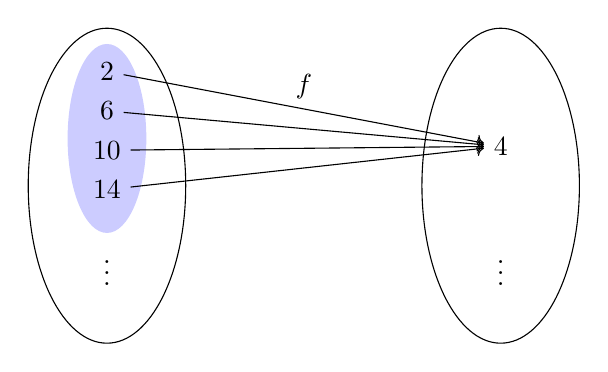
\begin{tikzpicture}
\draw (0,0) ellipse (1cm and 2cm);
\draw (5,0) circle (1cm and 2cm);
\fill[blue!20!white] (0,0.6) ellipse (0.5cm and 1.2cm);
\node (a) at (0,1.45) {2};
\node (b) at (0,0.95) {6};
\node (c) at (0,0.45) {10};
\node (d) at (0,-0.05) {14};
\node (t) at (5,0.5) {4};
\node at (0,-1) {$\vdots$};
\node at (5,-1) {$\vdots$};
\draw[->] (a) to node [above] {$f$} (t);
\draw[->] (b) -- (t);
\draw[->] (c) -- (t);
\draw[->] (d) -- (t);
\end{tikzpicture}
\end{center}
\caption{\label{fig:preimage}The pre-image of 4 under $f(x) = 7^x \mod 15$.}
\end{figure}

\paragraph*{Retrodictive Executions, Function Pre-images, and NP-Complete Problems.}
We now express the computational problems above uniformly as queries
over function pre-images. Given finite sets $A$ and $B$, a function $f
: A \rightarrow B$ and an element $y \in B$, we define $\preim{f}{y}$,
the pre-image of $y$ under $f$, as the set $\{ x \in A ~|~ f(x) = y
\}$. For example, let $A = B = \{0,1,\ldots,15\}$ and let $f(x) = 7^x
\mod 15$, then the collection of values that $f$ maps to 4,
$\preim{f}{4}$, is the set $\{ 2, 6, 10, 14 \}$.

Referring back to Fig.~\ref{fig:templateQC}, we observe that the
quantum algorithm can be decomposed into: (a) the computation up to
step (3) which just computes the pre-image of the ancilla measurement
under $f$, and (b) a module performing Hadamard of QFT to analyze this
pre-image. For example, the pre-image of 4 under $f(x) = 7^x \mod 15$
displayed in Fig.~\ref{fig:preimage} would be represented as the
superposition $\ket{\psi} = 1/2 (\ket{2} + \ket{6} + \ket{10} +
\ket{14})$ at step (3) of Shor's algorithm. What is crucial is that
although the quantum state $\ket{\psi}$ is not directly observable,
this is of no concern. Shor's algorithm does not actually care about
the full description of the pre-image, only about a global property of
the pre-image: its period. Indeed, in the quantum algorithms we
discussed, the full calculation of pre-image is never needed: each
algorithm computes a particular global property of the corresponding
pre-image. The Deutsch and Deutsch-Jozsa algorithms only need to
distinguish whether the pre-image of either 1 or 0 is empty, contains
half the elements, or the entire set. The Bernstein-Vazirani algorithm
only needs $n$ queries over the pre-image of either 1 or 0: query $i$
asks whether $2^i$ is a member of the pre-image and the answer
determines bit $i$ of the secret $s$. Indeed, by definition, $f(2^i) =
s_i$ and hence $s_i$ is 1 iff $2^i$ is a member of the pre-image of
1. In the case of the Simon problem, we calculate $f(x) = w$ for some
$x$ and query the pre-image of $w$ to get the other value in the
pre-image.

To summarize, quantum algorithms compute ``simple queries'' over
pre-images, and in fact, unless $P=NP$, such simple queries are the
only possibility since the full calculation of a pre-image is an
NP-complete problem, and it is believed that even full fledged quantum
computers cannot solve NP-complete problems. To appreciate the
difficulty of computing pre-images in general, note that finding the
pre-image of a function is subsumes several challenging computational
problems such as pre-image attacks on hash
functions~\cite{10.1007/978-3-540-25937-4_24}, predicting
environmental conditions that allow certain reactions to take place in
computational biology~\cite{Klotz2013,akutsu2009analyses}, and finding
the pre-image of feature vectors in the space induced by a kernel in
neural networks~\cite{1353287}. More to the point, the boolean
satisfiability problem SAT is expressible as a boolean function over
the input variables and solving a SAT problem is asking for the
pre-image of \textsf{true}. Indeed, based on the conjectured existence
of one-way functions which itself implies $\mathit{P} \neq
\mathit{NP}$, all these pre-images calculations are believed to be
computationally intractable in their most general setting.

The obvious question to ask now is whether the retrodictive execution
can be tuned to only produce the required statistics instead producing
the full description of pre-images. 

\newpage





insight 1: qft does not care about 0+2+4.... vs 1+3+5....

0 0 ?
0 1 ?
1 0 ?
1 1 ?

equiv no matter what ? is
? is used in the computation (don't care about value)
others not used
so we just need to keep track of which vars are used

run experiments with PEX and PEY





2. Hadamard basis: Tofffoli + Hadamard is universal so we “just” need to understand how to run in X basis. 

   Get rid of all quantum gates and run just the reversible classical part but with different taint analyses

   Essentially we have two colors and we do taint analysis

   Blue and Red; when blue interacts with red it gets tainted

   We have two operations +red (add red) -red (remove red)

   Remember cx(+,-) = (-,-) 

   Some interactions (Toffoli) want to create more refined operations +/-(1/2)(red) +/-(red)
   The more you do these operations the more precise it wants to be +/-(1/4)(red) +/-(1/2) red +/-(red)

   And so on

   You can truncate at the desired level of accuracy

   The taint analysis groups variables in “waves” (superpositions) of things that have the same color so the values we

     propagate are “red: phase=p; frequency=f; involved variables={x1,x2,…}”

   Seems that naive taint analysis is just keep track of which variable is used



------------

run again; refined pe; var used; if used twice then disappears

go back to that stupid paper about logic programming and xor 

The equations turn out to be trivial when the period is a power of
2. This occurs when the number to factor is a product of Fermat
primes: 3, 5, 17, 257, 65537, \ldots. The equations generated for some
of these cases are in Fig.~\ref{fig:shor2-eqs}. 


need stats only
PEX , PEY ...

core of many quantum algos is quantum oracle uf
two inputs; two outputs
system; ancilla;
normal eval; control ancilla; system unknown; so throw in complete superposition and
eval forward

\paragraph*{Retrodictive QFT.}

only need number of vars !!!!

solve other problems with just knowing which vars are involved

\paragraph*{Discussion.}

   Normal quantum evolution: from present to future

   Now what if I had partial knowledge about the future; what can you
   say about the present?  (And then about the rest of the unknown
   future)

   Can this help flow of information, complexity, etc?  

   In some cases, partial knowledge about the future is enough to
   predict the present accurately enough

   to then predict everything about the future; in some cases it is not enough

   Possibility that collapse of wave function is information flow back
   from measured future to present unknown initial conditions and then
   back to rest of wave that was not measured


Provide a general introduction to the topic and a brief non-technical
summary of your main results and their implication.

200 words ??

main text
  2000-2500 words
  3-4 figures
  30-50 references

Methods section
  3000 words
  more references ok
  
Author contributions

Code available  

https://quantumalgorithmzoo.org

every quantum circuit can be written using Toffoli and Hadamard
retro just go through Toffoli; ignore Had; but of course we are using symbolic eval

can H be moved past Toffoli?

universe uses lazy evaluation?

algebra of Toffoli and Hadamard
ZX calculus

fourier transform classical efficient in some cases

Ewin Tang papers

kochen specker ??

\printbibliography[heading=subbibliography]
\end{refsection}

%%%%%%%%%%%%%%%%%%%%%%%%%%%%%%%%%%%%%%%%%%%%%%%%%%%%%%%%%%%%%%%%%%%%%%%%%%%%%%%%%%%%%%%%%%
\section{Methods}

%% 3000 words but could be longer

\begin{refsection}

\paragraph*{Lazy Evaluation.}
Consider a program that searches for three different numbers $x$, $y$,
and $z$ each in the range $[1..n]$ and that sum to $s$. A
well-established design principle for solving such problems is the
\emph{generate-and-test} computational paradigm. Following this
principle, a simple program to solve this problem in the programming
language Haskell is:

\begin{verbatim}
generate :: Int -> [(Int,Int,Int)]
generate n =  [(x,y,z) | x <- [1..n], y <- [1..n], z <- [1..n]]

test :: Int -> [(Int,Int,Int)] -> [(Int,Int,Int)]
test s nums = [(x,y,z) | (x,y,z) <- nums, x /= y, x /= z, y /= z, x+y+z == s]

find :: Int -> Int -> (Int,Int,Int)
find s =  head . test s . generate
\end{verbatim}

The program consists of three functions: \verb|generate| that produces
all triples \verb|(x,y,z)| from \verb|(1,1,1)| to \verb|(n,n,n)|;
\verb|test| that checks that the numbers are different and that their
sum is equal to \verb|s|; and \verb|find| that composes the two
functions: generating all triples, testing the ones that satisfy the
condition, and returning the first solution. Running this program to
find numbers in the range $[1..6]$ that sum to 15 immediately produces
$(4,5,6)$ as expected.

But what if the range of interest was $[1..10000000]$ ? A na\"\i ve
execution of the generate-and-test method would be prohibitively
expensive as it would spend all its time generating an enormous number
of triples that are un-needed. Lazy demand-driven evaluation as
implemented in Haskell succeeds in a few seconds with the result
$(1,2,12)$, however. The idea is simple: instead of eagerly generating
all the triples, generate a process that, when queried, produces one
triple at a time on demand. Conceptually the execution starts from the
observer site which is asking for the first element of a list; this
demand is propagated to the function \verb|test| which itself
propagates the demand to the function \verb|generate|. As each triple
is generated, it is tested until one triple passes the test. This
triple is immediately returned without having to generate any
additional values.

\paragraph*{Partial Evaluation.}
Below is a Haskell program that computes $a^n$ by repeated squaring:
\begin{verbatim}
power :: Int -> Int -> Int
power a n
  | n == 0     = 1
  | n == 1     = a
  | even n     = let r = power a (n `div` 2) in r * r 
  | otherwise  = a * power a (n-1)
\end{verbatim}
When both inputs are known, e.g., \verb|a = 3| and \verb|n = 5|, the
program evaluates as follows:
\begin{verbatim}
   power 3 5
=  3 * power 3 4
=  3 * (let r1 = power 3 2 in r1 * r1)
=  3 * (let r1 = (let r2 = power 3 1 in r2 * r2) in r1 * r1)
=  3 * (let r1 = (let r2 = 3 in r2 * r2) in r1 * r1)
=  3 * (let r1 = 9 in r1 * r1)
=  243
\end{verbatim}

Partial evaluation is used when we only have partial information about
the inputs. Say we only know $n=5$. A partial evaluator then attempts
to evaluate \verb|power| with symbolic input \verb|a| and actual input
\verb|n=5|. This evaluation proceeds as follows:
\begin{verbatim}
   power a 5 
=  a * power a 4 
=  a * (let r1 = power a 2 in r1 * r1)
=  a * (let r1 = (let r2 = power a 1 in r2 * r2) in r1 * r1)
=  a * (let r1 = (let r2 = a in r2 * r2) in r1 * r1)
=  a * (let r1 = a * a in r1 * r1)
=  let r1 = a * a in a * r1 * r1
\end{verbatim}
All of this evaluation, simplification, and specialization happens
without knowledge of \verb|a|. Just knowing \verb|n| was enough to
produce a residual program that is much simpler. 






The evolution of a quantum system is typically understood as
proceeding forwards in time --- from the present to the future. As
shown in Fig.~\ref{fig:templateQC}(a), 

Since the conventional execution starts with complete ignorance about
the future, the initial state is prepared as a superposition that
includes every possibility. In a well-designed algorithm, , by the
time the computation reaches the measurement stages, the relative
phases and probability amplitudes in that enormous superposition have
become biased towards states of interest which are projected to
produce the final answer.

\paragraph*{Data Availability.} available 

\paragraph*{Discussion.}
Possibility that collapse of wave function is information flow back
from measured future to present unknown initial conditions and then
back to rest of wave that was not measured

transactional interpretation?

Luckily, the problems of concern to us are quite special: (i) the
functions are not arbitrary but have additional structure that can be
exploited, and (ii) we never need access to all the elements in the
pre-image; we just need to answer aggregate queries about the
pre-images. Quantum algorithms somehow exploit these properties along
with some physical principles to solve these problems efficiently. To
understand the precise way in which this is happening, we start with
the template of the quantum circuit used for solving all the problems
above in Fig.~\ref{fig:templateQC}.

The core of the circuit is the $U_f$ block which can be assumed to be
implemented using only generalized Toffoli gates. The block implements
the unitary transformation: $U_f(\ket{x}\ket{y}) = \ket{x}\ket{f(x)
  \oplus y}$ where $\oplus$ is the (bitwise) exclusive-or operation;
it defines the function of interest whose pre-image properties are to
be calculated. The inputs of the $U_f$ block are grouped in two
registers: the top register contains an equal superposition of all
possible inputs to $f$; the second register is prepared in initial
states that depend on the specific algorithm. Thus, the state at slice
(1) in the figure is:
  \[
  \frac{1}{\sqrt{2^n}\sqrt{2^m}}\sum_{x=0}^{2^n-1} ~\sum_{y=0}^{2^m-1} ~\ket{x}\ket{y}
  \]
This is transformed by $U_f$ to:
  \[
  \frac{1}{\sqrt{2^n}\sqrt{2^m}}
  \sum_{x=0}^{2^n-1} ~\sum_{y=0}^{2^m-1} ~\ket{x}\ket{f(x)\oplus y}
  \]
So far, nothing too interesting is happening: we have just produced a
superposition of states where each state is a possible input to $f$,
say $x$, tensored with $f(x) \oplus y$, the result of applying $f$ to
this particular input adjusted by the second register $y$. At slice
(3), something remarkable occurs; the result $w$ of measuring the
second register ``kicks back'' information to the first register whose
state becomes a superposition of those values $x$ that are consistent
with the measurement, i.e., \emph{the pre-image of $w$ under $f$!}
That pre-image representation is then analyzed using the Quantum
Fourier Transform (QFT) to produce the final result.

Quantum algorithms typically operate on a \emph{black box} holding a
classical function whose properties need to be computed. The general
structure of these algorithms is to (i) create a superposition of
values to be passed as inputs to the black box, (ii) apply the
operation inside the black box, and (iii) post-process the output of
the black box. We observe that, in quite a few cases, steps (i) and
(iii) are actually unnecessary and that the entire ``quantum''
algorithm can be executed by forward or backward, full or partial,
efficient classical \emph{symbolic execution} of the black box.


typical use: superposition, Uf, measure second register; we only care
about which x has f(x) = r

By default all functions are reversible. 

To make them irreversible you fix h and delete g. If you delete too
much the function becomes very expensive to reverse. So one way
functions emerge


simplify function has polynomial realization and we want
statistics about the kernel (not necessarily compute it exactly)



collect assumptions:


important that no matter what measurement we do on w, properly we want is the same


since we say that algos related to pre-images lets do naive thing and eval backwards

assumptions we have a rev circuit efficient forward
two inputs: first is full superposition; second whatever
first output same as first input; but that is only at point 2; at point 3 explain kick back; misleading to think it is the same after 3
second output is result of function; measure; have element of range; go back with that elem
if we knew first output as well as w then eval backwards same complexity but we only know w and we don't know first output; because we are starting at 3 not 2

we have no use for H block; it was only there for the forward exec to express our complete ignorance o the future; prepared with every x but if we have knowledge about future (w measured) we go back to find the values of x in the present that would be consistent with w so general circuit reduces to :

...

fix pics to have amplitudes with y (most general)

To what extent are the quantum algorithms above taking advantage of
non-classical features. We posit that pre-image computation can be, at
least for some of the some of the algorithms, be performed
classically. The main insight needed for that is to perform the
execution \emph{symbolically}. We illustrate the idea with two
examples.

We need to explain ideas about time-reversal, prediction and retrodiction in 
physics. The laws of computation and the laws of physics are intimately related. 
When does knowing something about the future help us unveil the structure or 
symmetries of the past? It is like a detective story, but one with 
ramifications in complexity and/or efficiency. Problems involving questions 
where answers demand a Many(past)-to-one(future) map are at the root of 
our proposal.... {\color{red} Difference between exploiting or not entanglement
in the unitary evolution.}

As we demonstrate, the family of quantum algorithms initiated by
Deutsch's algorithm and culminating with Shor's algorithm (i) solves
variants of the pre-image problem efficiently, and, in that context,
(ii) answering queries about pre-images is closely related to
\emph{retrodictive quantum theory}~\cite{sym13040586},
retrocausality~\cite{Aharonov2008}, and the time-symmetry of physical
laws~\cite{RevModPhys.27.179}.


\begin{itemize}
\item Retrodictive execution more efficient in some cases. What cases?
\item Here are three examples: Deutsch-Jozsa, Simon, Shor when period
  is close to a power of 2
\item Symbolic (retrodictive) evaluation as a broader perspective to classical computation
\item Symbolic execution allows you to express/discover interference via shared variables
\item When interference pattern is simple symbolic execution reveals
  solutions faster (and completely classically)
\item Symbolic execution as a “classical waves” computing paradigm
\end{itemize}


to represent unequal superpositions do multiple runs with vars the
first has x1 x2 etc the second has y1 2y2 etc or y2/2 etc, or with
various patterns of negative weights.... And then the punchline would
be to interpret the negative backwards. So instead of all forward or
all retro we have some values going forward and then backwards

Start with the story about function many to one etc why superpositions
because we don’t know which values so we try all easy to represent by
unknown vars so we can represent superpositions as vars and equations
between them but at the end we want stats about superpositions slow
way is to generate all equations and solve faster way is generate many
sets of equations with different weights and sum to get your stats


\paragraph*{Partial Symbolic Evaluation with Algebraic Normal Form (ANF).}

The resulting
expressions are in algebraic normal form~\cite{TOKAREVA20151} where
$+$ denotes exclusive-or. 

We should use two prototypical examples to illustrate main ideas
before going to the complex ones. The examples I have in mind are:
Deutsch-Jozsa and Simon (precursor of Shor's). There are prior works
on de-quantization of the first problem and should make contact with
their resolution. Perhaps we can show that they are as efficient
classically? That would justify retrodiction alone. The more complex
(and important) case of factorization should be the natural follow up.

The idea of symbolic execution is not tied to forward or backward
execution. We should introduce it in a way that is independent of the
direction of execution. What the idea depends on however is that the
wave function, at least in the cases we are considering, can be
represented as equations over booleans.

Wave Functions as Equations over Booleans

in the typical scenario for using quantum oracles, we can represent
wave function as equations over booleans; equations represent the wave
function but the solution is unobservable just like the components of
the superposition in the wave function are not observable; just like
we don't directly get access to the components of the wave function;
we don't directly get access to the solution of the equations; need to
"observe" the equations

we can go backwards with an equation (representing a wave function
sigma x where f(x) = r and go back towards the present to calculate
the wave function (represented as equations again)

Musing: how to explain complementarity when wave function is
represented as an equation? Kochen specker;
 
or contextuality
 
observer 1 measures wires a,b; obs2 measures wires b,c; not commuting;
each obs gives partial solution to equations; but partial solutions
cannot lead to a global solution
 
KS suggests that equations do not have unique solutions; only
materialize when you measure;

can associate a probability with each variable in a equation: look at
all solutions and see the contribution of each variable to these
solutions.

\paragraph*{Complexity Analysis.}
one pass over circuit BUT complexity of normalizing to ANF not trivial; be careful

\paragraph*{Supplementary Information.} 
\label{par:shor21}

Equations generated by retrodictive execution of $4^x \mod{21}$
starting from observed result 1 and unknown $x$. The circuit consists
of 9 qubits, 36400 \cx-gates, 38200 \ccx-gates, and 4000
\cccx-gates. There are only three equations but each equation is
exponentially large.

$1 \oplus x_0 \oplus x_0x_1x_2 \oplus x_0x_1x_2x_3x_4 \oplus x_0x_1x_2x_3x_4x_5x_6 \oplus x_0x_1x_2x_3x_4x_5x_6x_7x_8 \oplus
 x_0x_1x_2x_3x_4x_5x_6x_7x_9 \oplus x_0x_1x_2x_3x_4x_5x_6x_8 \oplus x_0x_1x_2x_3x_4x_5x_6x_8x_9 \oplus
 x_0x_1x_2x_3x_4x_5x_7 \oplus x_0x_1x_2x_3x_4x_5x_7x_8x_9 \oplus x_0x_1x_2x_3x_4x_5x_7x_9 \oplus
 x_0x_1x_2x_3x_4x_5x_8 \oplus x_0x_1x_2x_3x_4x_5x_9 \oplus x_0x_1x_2x_3x_4x_6 \oplus x_0x_1x_2x_3x_4x_6x_7 \oplus
 x_0x_1x_2x_3x_4x_6x_7x_8 \oplus x_0x_1x_2x_3x_4x_6x_7x_8x_9 \oplus x_0x_1x_2x_3x_4x_6x_8x_9 \oplus
 x_0x_1x_2x_3x_4x_6x_9 \oplus x_0x_1x_2x_3x_4x_7x_8 \oplus x_0x_1x_2x_3x_4x_7x_9 \oplus x_0x_1x_2x_3x_4x_8 \oplus
 x_0x_1x_2x_3x_4x_8x_9 \oplus x_0x_1x_2x_3x_5 \oplus x_0x_1x_2x_3x_5x_6x_7 \oplus x_0x_1x_2x_3x_5x_6x_7x_8x_9 \oplus
 x_0x_1x_2x_3x_5x_6x_7x_9 \oplus x_0x_1x_2x_3x_5x_6x_8 \oplus x_0x_1x_2x_3x_5x_6x_9 \oplus x_0x_1x_2x_3x_5x_7 \oplus
 x_0x_1x_2x_3x_5x_7x_8 \oplus x_0x_1x_2x_3x_5x_7x_8x_9 \oplus x_0x_1x_2x_3x_5x_8x_9 \oplus x_0x_1x_2x_3x_5x_9 \oplus
 x_0x_1x_2x_3x_6 \oplus x_0x_1x_2x_3x_6x_7x_8 \oplus x_0x_1x_2x_3x_6x_7x_9 \oplus x_0x_1x_2x_3x_6x_8 \oplus
 x_0x_1x_2x_3x_6x_8x_9 \oplus x_0x_1x_2x_3x_7 \oplus x_0x_1x_2x_3x_7x_8x_9 \oplus x_0x_1x_2x_3x_7x_9 \oplus
 x_0x_1x_2x_3x_8 \oplus x_0x_1x_2x_3x_9 \oplus x_0x_1x_2x_4 \oplus x_0x_1x_2x_4x_5 \oplus x_0x_1x_2x_4x_5x_6 \oplus
 x_0x_1x_2x_4x_5x_6x_7 \oplus x_0x_1x_2x_4x_5x_6x_7x_8 \oplus x_0x_1x_2x_4x_5x_6x_7x_8x_9 \oplus
 x_0x_1x_2x_4x_5x_6x_8x_9 \oplus x_0x_1x_2x_4x_5x_6x_9 \oplus x_0x_1x_2x_4x_5x_7x_8 \oplus x_0x_1x_2x_4x_5x_7x_9 \oplus
 x_0x_1x_2x_4x_5x_8 \oplus x_0x_1x_2x_4x_5x_8x_9 \oplus x_0x_1x_2x_4x_6x_7 \oplus x_0x_1x_2x_4x_6x_7x_8x_9 \oplus
 x_0x_1x_2x_4x_6x_7x_9 \oplus x_0x_1x_2x_4x_6x_8 \oplus x_0x_1x_2x_4x_6x_9 \oplus x_0x_1x_2x_4x_7 \oplus
 x_0x_1x_2x_4x_7x_8 \oplus x_0x_1x_2x_4x_7x_8x_9 \oplus x_0x_1x_2x_4x_8x_9 \oplus x_0x_1x_2x_4x_9 \oplus
 x_0x_1x_2x_5x_6 \oplus x_0x_1x_2x_5x_6x_7x_8 \oplus x_0x_1x_2x_5x_6x_7x_9 \oplus x_0x_1x_2x_5x_6x_8 \oplus
 x_0x_1x_2x_5x_6x_8x_9 \oplus x_0x_1x_2x_5x_7 \oplus x_0x_1x_2x_5x_7x_8x_9 \oplus x_0x_1x_2x_5x_7x_9 \oplus
 x_0x_1x_2x_5x_8 \oplus x_0x_1x_2x_5x_9 \oplus x_0x_1x_2x_6 \oplus x_0x_1x_2x_6x_7 \oplus x_0x_1x_2x_6x_7x_8 \oplus
 x_0x_1x_2x_6x_7x_8x_9 \oplus x_0x_1x_2x_6x_8x_9 \oplus x_0x_1x_2x_6x_9 \oplus x_0x_1x_2x_7x_8 \oplus x_0x_1x_2x_7x_9
 \oplus x_0x_1x_2x_8 \oplus x_0x_1x_2x_8x_9 \oplus x_0x_1x_3 \oplus x_0x_1x_3x_4x_5 \oplus x_0x_1x_3x_4x_5x_6x_7 \oplus
 x_0x_1x_3x_4x_5x_6x_7x_8x_9 \oplus x_0x_1x_3x_4x_5x_6x_7x_9 \oplus x_0x_1x_3x_4x_5x_6x_8 \oplus
 x_0x_1x_3x_4x_5x_6x_9 \oplus x_0x_1x_3x_4x_5x_7 \oplus x_0x_1x_3x_4x_5x_7x_8 \oplus x_0x_1x_3x_4x_5x_7x_8x_9 \oplus
 x_0x_1x_3x_4x_5x_8x_9 \oplus x_0x_1x_3x_4x_5x_9 \oplus x_0x_1x_3x_4x_6 \oplus x_0x_1x_3x_4x_6x_7x_8 \oplus
 x_0x_1x_3x_4x_6x_7x_9 \oplus x_0x_1x_3x_4x_6x_8 \oplus x_0x_1x_3x_4x_6x_8x_9 \oplus x_0x_1x_3x_4x_7 \oplus
 x_0x_1x_3x_4x_7x_8x_9 \oplus x_0x_1x_3x_4x_7x_9 \oplus x_0x_1x_3x_4x_8 \oplus x_0x_1x_3x_4x_9 \oplus x_0x_1x_3x_5 \oplus
 x_0x_1x_3x_5x_6 \oplus x_0x_1x_3x_5x_6x_7 \oplus x_0x_1x_3x_5x_6x_7x_8 \oplus x_0x_1x_3x_5x_6x_7x_8x_9 \oplus
 x_0x_1x_3x_5x_6x_8x_9 \oplus x_0x_1x_3x_5x_6x_9 \oplus x_0x_1x_3x_5x_7x_8 \oplus x_0x_1x_3x_5x_7x_9 \oplus
 x_0x_1x_3x_5x_8 \oplus x_0x_1x_3x_5x_8x_9 \oplus x_0x_1x_3x_6x_7 \oplus x_0x_1x_3x_6x_7x_8x_9 \oplus
 x_0x_1x_3x_6x_7x_9 \oplus x_0x_1x_3x_6x_8 \oplus x_0x_1x_3x_6x_9 \oplus x_0x_1x_3x_7 \oplus x_0x_1x_3x_7x_8 \oplus
 x_0x_1x_3x_7x_8x_9 \oplus x_0x_1x_3x_8x_9 \oplus x_0x_1x_3x_9 \oplus x_0x_1x_4 \oplus x_0x_1x_4x_5x_6 \oplus
 x_0x_1x_4x_5x_6x_7x_8 \oplus x_0x_1x_4x_5x_6x_7x_9 \oplus x_0x_1x_4x_5x_6x_8 \oplus x_0x_1x_4x_5x_6x_8x_9 \oplus
 x_0x_1x_4x_5x_7 \oplus x_0x_1x_4x_5x_7x_8x_9 \oplus x_0x_1x_4x_5x_7x_9 \oplus x_0x_1x_4x_5x_8 \oplus x_0x_1x_4x_5x_9
 \oplus x_0x_1x_4x_6 \oplus x_0x_1x_4x_6x_7 \oplus x_0x_1x_4x_6x_7x_8 \oplus x_0x_1x_4x_6x_7x_8x_9 \oplus
 x_0x_1x_4x_6x_8x_9 \oplus x_0x_1x_4x_6x_9 \oplus x_0x_1x_4x_7x_8 \oplus x_0x_1x_4x_7x_9 \oplus x_0x_1x_4x_8 \oplus
 x_0x_1x_4x_8x_9 \oplus x_0x_1x_5 \oplus x_0x_1x_5x_6x_7 \oplus x_0x_1x_5x_6x_7x_8x_9 \oplus x_0x_1x_5x_6x_7x_9 \oplus
 x_0x_1x_5x_6x_8 \oplus x_0x_1x_5x_6x_9 \oplus x_0x_1x_5x_7 \oplus x_0x_1x_5x_7x_8 \oplus x_0x_1x_5x_7x_8x_9 \oplus
 x_0x_1x_5x_8x_9 \oplus x_0x_1x_5x_9 \oplus x_0x_1x_6 \oplus x_0x_1x_6x_7x_8 \oplus x_0x_1x_6x_7x_9 \oplus x_0x_1x_6x_8 \oplus
 x_0x_1x_6x_8x_9 \oplus x_0x_1x_7 \oplus x_0x_1x_7x_8x_9 \oplus x_0x_1x_7x_9 \oplus x_0x_1x_8 \oplus x_0x_1x_9 \oplus x_0x_2
 \oplus x_0x_2x_3 \oplus x_0x_2x_3x_4 \oplus x_0x_2x_3x_4x_5 \oplus x_0x_2x_3x_4x_5x_6 \oplus x_0x_2x_3x_4x_5x_6x_7 \oplus
 x_0x_2x_3x_4x_5x_6x_7x_8 \oplus x_0x_2x_3x_4x_5x_6x_7x_8x_9 \oplus x_0x_2x_3x_4x_5x_6x_8x_9 \oplus
 x_0x_2x_3x_4x_5x_6x_9 \oplus x_0x_2x_3x_4x_5x_7x_8 \oplus x_0x_2x_3x_4x_5x_7x_9 \oplus x_0x_2x_3x_4x_5x_8 \oplus
 x_0x_2x_3x_4x_5x_8x_9 \oplus x_0x_2x_3x_4x_6x_7 \oplus x_0x_2x_3x_4x_6x_7x_8x_9 \oplus x_0x_2x_3x_4x_6x_7x_9 \oplus
 x_0x_2x_3x_4x_6x_8 \oplus x_0x_2x_3x_4x_6x_9 \oplus x_0x_2x_3x_4x_7 \oplus x_0x_2x_3x_4x_7x_8 \oplus
 x_0x_2x_3x_4x_7x_8x_9 \oplus x_0x_2x_3x_4x_8x_9 \oplus x_0x_2x_3x_4x_9 \oplus x_0x_2x_3x_5x_6 \oplus
 x_0x_2x_3x_5x_6x_7x_8 \oplus x_0x_2x_3x_5x_6x_7x_9 \oplus x_0x_2x_3x_5x_6x_8 \oplus x_0x_2x_3x_5x_6x_8x_9 \oplus
 x_0x_2x_3x_5x_7 \oplus x_0x_2x_3x_5x_7x_8x_9 \oplus x_0x_2x_3x_5x_7x_9 \oplus x_0x_2x_3x_5x_8 \oplus x_0x_2x_3x_5x_9
 \oplus x_0x_2x_3x_6 \oplus x_0x_2x_3x_6x_7 \oplus x_0x_2x_3x_6x_7x_8 \oplus x_0x_2x_3x_6x_7x_8x_9 \oplus
 x_0x_2x_3x_6x_8x_9 \oplus x_0x_2x_3x_6x_9 \oplus x_0x_2x_3x_7x_8 \oplus x_0x_2x_3x_7x_9 \oplus x_0x_2x_3x_8 \oplus
 x_0x_2x_3x_8x_9 \oplus x_0x_2x_4x_5 \oplus x_0x_2x_4x_5x_6x_7 \oplus x_0x_2x_4x_5x_6x_7x_8x_9 \oplus
 x_0x_2x_4x_5x_6x_7x_9 \oplus x_0x_2x_4x_5x_6x_8 \oplus x_0x_2x_4x_5x_6x_9 \oplus x_0x_2x_4x_5x_7 \oplus
 x_0x_2x_4x_5x_7x_8 \oplus x_0x_2x_4x_5x_7x_8x_9 \oplus x_0x_2x_4x_5x_8x_9 \oplus x_0x_2x_4x_5x_9 \oplus x_0x_2x_4x_6
 \oplus x_0x_2x_4x_6x_7x_8 \oplus x_0x_2x_4x_6x_7x_9 \oplus x_0x_2x_4x_6x_8 \oplus x_0x_2x_4x_6x_8x_9 \oplus x_0x_2x_4x_7
 \oplus x_0x_2x_4x_7x_8x_9 \oplus x_0x_2x_4x_7x_9 \oplus x_0x_2x_4x_8 \oplus x_0x_2x_4x_9 \oplus x_0x_2x_5 \oplus x_0x_2x_5x_6
 \oplus x_0x_2x_5x_6x_7 \oplus x_0x_2x_5x_6x_7x_8 \oplus x_0x_2x_5x_6x_7x_8x_9 \oplus x_0x_2x_5x_6x_8x_9 \oplus
 x_0x_2x_5x_6x_9 \oplus x_0x_2x_5x_7x_8 \oplus x_0x_2x_5x_7x_9 \oplus x_0x_2x_5x_8 \oplus x_0x_2x_5x_8x_9 \oplus
 x_0x_2x_6x_7 \oplus x_0x_2x_6x_7x_8x_9 \oplus x_0x_2x_6x_7x_9 \oplus x_0x_2x_6x_8 \oplus x_0x_2x_6x_9 \oplus x_0x_2x_7 \oplus
 x_0x_2x_7x_8 \oplus x_0x_2x_7x_8x_9 \oplus x_0x_2x_8x_9 \oplus x_0x_2x_9 \oplus x_0x_3x_4 \oplus x_0x_3x_4x_5x_6 \oplus
 x_0x_3x_4x_5x_6x_7x_8 \oplus x_0x_3x_4x_5x_6x_7x_9 \oplus x_0x_3x_4x_5x_6x_8 \oplus x_0x_3x_4x_5x_6x_8x_9 \oplus
 x_0x_3x_4x_5x_7 \oplus x_0x_3x_4x_5x_7x_8x_9 \oplus x_0x_3x_4x_5x_7x_9 \oplus x_0x_3x_4x_5x_8 \oplus x_0x_3x_4x_5x_9
 \oplus x_0x_3x_4x_6 \oplus x_0x_3x_4x_6x_7 \oplus x_0x_3x_4x_6x_7x_8 \oplus x_0x_3x_4x_6x_7x_8x_9 \oplus
 x_0x_3x_4x_6x_8x_9 \oplus x_0x_3x_4x_6x_9 \oplus x_0x_3x_4x_7x_8 \oplus x_0x_3x_4x_7x_9 \oplus x_0x_3x_4x_8 \oplus
 x_0x_3x_4x_8x_9 \oplus x_0x_3x_5 \oplus x_0x_3x_5x_6x_7 \oplus x_0x_3x_5x_6x_7x_8x_9 \oplus x_0x_3x_5x_6x_7x_9 \oplus
 x_0x_3x_5x_6x_8 \oplus x_0x_3x_5x_6x_9 \oplus x_0x_3x_5x_7 \oplus x_0x_3x_5x_7x_8 \oplus x_0x_3x_5x_7x_8x_9 \oplus
 x_0x_3x_5x_8x_9 \oplus x_0x_3x_5x_9 \oplus x_0x_3x_6 \oplus x_0x_3x_6x_7x_8 \oplus x_0x_3x_6x_7x_9 \oplus x_0x_3x_6x_8 \oplus
 x_0x_3x_6x_8x_9 \oplus x_0x_3x_7 \oplus x_0x_3x_7x_8x_9 \oplus x_0x_3x_7x_9 \oplus x_0x_3x_8 \oplus x_0x_3x_9 \oplus x_0x_4
 \oplus x_0x_4x_5 \oplus x_0x_4x_5x_6 \oplus x_0x_4x_5x_6x_7 \oplus x_0x_4x_5x_6x_7x_8 \oplus x_0x_4x_5x_6x_7x_8x_9 \oplus
 x_0x_4x_5x_6x_8x_9 \oplus x_0x_4x_5x_6x_9 \oplus x_0x_4x_5x_7x_8 \oplus x_0x_4x_5x_7x_9 \oplus x_0x_4x_5x_8 \oplus
 x_0x_4x_5x_8x_9 \oplus x_0x_4x_6x_7 \oplus x_0x_4x_6x_7x_8x_9 \oplus x_0x_4x_6x_7x_9 \oplus x_0x_4x_6x_8 \oplus
 x_0x_4x_6x_9 \oplus x_0x_4x_7 \oplus x_0x_4x_7x_8 \oplus x_0x_4x_7x_8x_9 \oplus x_0x_4x_8x_9 \oplus x_0x_4x_9 \oplus
 x_0x_5x_6 \oplus x_0x_5x_6x_7x_8 \oplus x_0x_5x_6x_7x_9 \oplus x_0x_5x_6x_8 \oplus x_0x_5x_6x_8x_9 \oplus x_0x_5x_7 \oplus
 x_0x_5x_7x_8x_9 \oplus x_0x_5x_7x_9 \oplus x_0x_5x_8 \oplus x_0x_5x_9 \oplus x_0x_6 \oplus x_0x_6x_7 \oplus x_0x_6x_7x_8 \oplus
 x_0x_6x_7x_8x_9 \oplus x_0x_6x_8x_9 \oplus x_0x_6x_9 \oplus x_0x_7x_8 \oplus x_0x_7x_9 \oplus x_0x_8 \oplus x_0x_8x_9 \oplus x_1
 \oplus x_1x_2x_3 \oplus x_1x_2x_3x_4x_5 \oplus x_1x_2x_3x_4x_5x_6x_7 \oplus x_1x_2x_3x_4x_5x_6x_7x_8x_9 \oplus
 x_1x_2x_3x_4x_5x_6x_7x_9 \oplus x_1x_2x_3x_4x_5x_6x_8 \oplus x_1x_2x_3x_4x_5x_6x_9 \oplus x_1x_2x_3x_4x_5x_7 \oplus
 x_1x_2x_3x_4x_5x_7x_8 \oplus x_1x_2x_3x_4x_5x_7x_8x_9 \oplus x_1x_2x_3x_4x_5x_8x_9 \oplus x_1x_2x_3x_4x_5x_9 \oplus
 x_1x_2x_3x_4x_6 \oplus x_1x_2x_3x_4x_6x_7x_8 \oplus x_1x_2x_3x_4x_6x_7x_9 \oplus x_1x_2x_3x_4x_6x_8 \oplus
 x_1x_2x_3x_4x_6x_8x_9 \oplus x_1x_2x_3x_4x_7 \oplus x_1x_2x_3x_4x_7x_8x_9 \oplus x_1x_2x_3x_4x_7x_9 \oplus
 x_1x_2x_3x_4x_8 \oplus x_1x_2x_3x_4x_9 \oplus x_1x_2x_3x_5 \oplus x_1x_2x_3x_5x_6 \oplus x_1x_2x_3x_5x_6x_7 \oplus
 x_1x_2x_3x_5x_6x_7x_8 \oplus x_1x_2x_3x_5x_6x_7x_8x_9 \oplus x_1x_2x_3x_5x_6x_8x_9 \oplus x_1x_2x_3x_5x_6x_9 \oplus
 x_1x_2x_3x_5x_7x_8 \oplus x_1x_2x_3x_5x_7x_9 \oplus x_1x_2x_3x_5x_8 \oplus x_1x_2x_3x_5x_8x_9 \oplus x_1x_2x_3x_6x_7
 \oplus x_1x_2x_3x_6x_7x_8x_9 \oplus x_1x_2x_3x_6x_7x_9 \oplus x_1x_2x_3x_6x_8 \oplus x_1x_2x_3x_6x_9 \oplus x_1x_2x_3x_7
 \oplus x_1x_2x_3x_7x_8 \oplus x_1x_2x_3x_7x_8x_9 \oplus x_1x_2x_3x_8x_9 \oplus x_1x_2x_3x_9 \oplus x_1x_2x_4 \oplus
 x_1x_2x_4x_5x_6 \oplus x_1x_2x_4x_5x_6x_7x_8 \oplus x_1x_2x_4x_5x_6x_7x_9 \oplus x_1x_2x_4x_5x_6x_8 \oplus
 x_1x_2x_4x_5x_6x_8x_9 \oplus x_1x_2x_4x_5x_7 \oplus x_1x_2x_4x_5x_7x_8x_9 \oplus x_1x_2x_4x_5x_7x_9 \oplus
 x_1x_2x_4x_5x_8 \oplus x_1x_2x_4x_5x_9 \oplus x_1x_2x_4x_6 \oplus x_1x_2x_4x_6x_7 \oplus x_1x_2x_4x_6x_7x_8 \oplus
 x_1x_2x_4x_6x_7x_8x_9 \oplus x_1x_2x_4x_6x_8x_9 \oplus x_1x_2x_4x_6x_9 \oplus x_1x_2x_4x_7x_8 \oplus x_1x_2x_4x_7x_9
 \oplus x_1x_2x_4x_8 \oplus x_1x_2x_4x_8x_9 \oplus x_1x_2x_5 \oplus x_1x_2x_5x_6x_7 \oplus x_1x_2x_5x_6x_7x_8x_9 \oplus
 x_1x_2x_5x_6x_7x_9 \oplus x_1x_2x_5x_6x_8 \oplus x_1x_2x_5x_6x_9 \oplus x_1x_2x_5x_7 \oplus x_1x_2x_5x_7x_8 \oplus
 x_1x_2x_5x_7x_8x_9 \oplus x_1x_2x_5x_8x_9 \oplus x_1x_2x_5x_9 \oplus x_1x_2x_6 \oplus x_1x_2x_6x_7x_8 \oplus
 x_1x_2x_6x_7x_9 \oplus x_1x_2x_6x_8 \oplus x_1x_2x_6x_8x_9 \oplus x_1x_2x_7 \oplus x_1x_2x_7x_8x_9 \oplus x_1x_2x_7x_9 \oplus
 x_1x_2x_8 \oplus x_1x_2x_9 \oplus x_1x_3 \oplus x_1x_3x_4 \oplus x_1x_3x_4x_5 \oplus x_1x_3x_4x_5x_6 \oplus
 x_1x_3x_4x_5x_6x_7 \oplus x_1x_3x_4x_5x_6x_7x_8 \oplus x_1x_3x_4x_5x_6x_7x_8x_9 \oplus x_1x_3x_4x_5x_6x_8x_9 \oplus
 x_1x_3x_4x_5x_6x_9 \oplus x_1x_3x_4x_5x_7x_8 \oplus x_1x_3x_4x_5x_7x_9 \oplus x_1x_3x_4x_5x_8 \oplus
 x_1x_3x_4x_5x_8x_9 \oplus x_1x_3x_4x_6x_7 \oplus x_1x_3x_4x_6x_7x_8x_9 \oplus x_1x_3x_4x_6x_7x_9 \oplus
 x_1x_3x_4x_6x_8 \oplus x_1x_3x_4x_6x_9 \oplus x_1x_3x_4x_7 \oplus x_1x_3x_4x_7x_8 \oplus x_1x_3x_4x_7x_8x_9 \oplus
 x_1x_3x_4x_8x_9 \oplus x_1x_3x_4x_9 \oplus x_1x_3x_5x_6 \oplus x_1x_3x_5x_6x_7x_8 \oplus x_1x_3x_5x_6x_7x_9 \oplus
 x_1x_3x_5x_6x_8 \oplus x_1x_3x_5x_6x_8x_9 \oplus x_1x_3x_5x_7 \oplus x_1x_3x_5x_7x_8x_9 \oplus x_1x_3x_5x_7x_9 \oplus
 x_1x_3x_5x_8 \oplus x_1x_3x_5x_9 \oplus x_1x_3x_6 \oplus x_1x_3x_6x_7 \oplus x_1x_3x_6x_7x_8 \oplus x_1x_3x_6x_7x_8x_9 \oplus
 x_1x_3x_6x_8x_9 \oplus x_1x_3x_6x_9 \oplus x_1x_3x_7x_8 \oplus x_1x_3x_7x_9 \oplus x_1x_3x_8 \oplus x_1x_3x_8x_9 \oplus
 x_1x_4x_5 \oplus x_1x_4x_5x_6x_7 \oplus x_1x_4x_5x_6x_7x_8x_9 \oplus x_1x_4x_5x_6x_7x_9 \oplus x_1x_4x_5x_6x_8 \oplus
 x_1x_4x_5x_6x_9 \oplus x_1x_4x_5x_7 \oplus x_1x_4x_5x_7x_8 \oplus x_1x_4x_5x_7x_8x_9 \oplus x_1x_4x_5x_8x_9 \oplus
 x_1x_4x_5x_9 \oplus x_1x_4x_6 \oplus x_1x_4x_6x_7x_8 \oplus x_1x_4x_6x_7x_9 \oplus x_1x_4x_6x_8 \oplus x_1x_4x_6x_8x_9 \oplus
 x_1x_4x_7 \oplus x_1x_4x_7x_8x_9 \oplus x_1x_4x_7x_9 \oplus x_1x_4x_8 \oplus x_1x_4x_9 \oplus x_1x_5 \oplus x_1x_5x_6 \oplus
 x_1x_5x_6x_7 \oplus x_1x_5x_6x_7x_8 \oplus x_1x_5x_6x_7x_8x_9 \oplus x_1x_5x_6x_8x_9 \oplus x_1x_5x_6x_9 \oplus
 x_1x_5x_7x_8 \oplus x_1x_5x_7x_9 \oplus x_1x_5x_8 \oplus x_1x_5x_8x_9 \oplus x_1x_6x_7 \oplus x_1x_6x_7x_8x_9 \oplus
 x_1x_6x_7x_9 \oplus x_1x_6x_8 \oplus x_1x_6x_9 \oplus x_1x_7 \oplus x_1x_7x_8 \oplus x_1x_7x_8x_9 \oplus x_1x_8x_9 \oplus x_1x_9
 \oplus x_2 \oplus x_2x_3x_4 \oplus x_2x_3x_4x_5x_6 \oplus x_2x_3x_4x_5x_6x_7x_8 \oplus x_2x_3x_4x_5x_6x_7x_9 \oplus
 x_2x_3x_4x_5x_6x_8 \oplus x_2x_3x_4x_5x_6x_8x_9 \oplus x_2x_3x_4x_5x_7 \oplus x_2x_3x_4x_5x_7x_8x_9 \oplus
 x_2x_3x_4x_5x_7x_9 \oplus x_2x_3x_4x_5x_8 \oplus x_2x_3x_4x_5x_9 \oplus x_2x_3x_4x_6 \oplus x_2x_3x_4x_6x_7 \oplus
 x_2x_3x_4x_6x_7x_8 \oplus x_2x_3x_4x_6x_7x_8x_9 \oplus x_2x_3x_4x_6x_8x_9 \oplus x_2x_3x_4x_6x_9 \oplus
 x_2x_3x_4x_7x_8 \oplus x_2x_3x_4x_7x_9 \oplus x_2x_3x_4x_8 \oplus x_2x_3x_4x_8x_9 \oplus x_2x_3x_5 \oplus x_2x_3x_5x_6x_7
 \oplus x_2x_3x_5x_6x_7x_8x_9 \oplus x_2x_3x_5x_6x_7x_9 \oplus x_2x_3x_5x_6x_8 \oplus x_2x_3x_5x_6x_9 \oplus x_2x_3x_5x_7
 \oplus x_2x_3x_5x_7x_8 \oplus x_2x_3x_5x_7x_8x_9 \oplus x_2x_3x_5x_8x_9 \oplus x_2x_3x_5x_9 \oplus x_2x_3x_6 \oplus
 x_2x_3x_6x_7x_8 \oplus x_2x_3x_6x_7x_9 \oplus x_2x_3x_6x_8 \oplus x_2x_3x_6x_8x_9 \oplus x_2x_3x_7 \oplus x_2x_3x_7x_8x_9
 \oplus x_2x_3x_7x_9 \oplus x_2x_3x_8 \oplus x_2x_3x_9 \oplus x_2x_4 \oplus x_2x_4x_5 \oplus x_2x_4x_5x_6 \oplus x_2x_4x_5x_6x_7
 \oplus x_2x_4x_5x_6x_7x_8 \oplus x_2x_4x_5x_6x_7x_8x_9 \oplus x_2x_4x_5x_6x_8x_9 \oplus x_2x_4x_5x_6x_9 \oplus
 x_2x_4x_5x_7x_8 \oplus x_2x_4x_5x_7x_9 \oplus x_2x_4x_5x_8 \oplus x_2x_4x_5x_8x_9 \oplus x_2x_4x_6x_7 \oplus
 x_2x_4x_6x_7x_8x_9 \oplus x_2x_4x_6x_7x_9 \oplus x_2x_4x_6x_8 \oplus x_2x_4x_6x_9 \oplus x_2x_4x_7 \oplus x_2x_4x_7x_8 \oplus
 x_2x_4x_7x_8x_9 \oplus x_2x_4x_8x_9 \oplus x_2x_4x_9 \oplus x_2x_5x_6 \oplus x_2x_5x_6x_7x_8 \oplus x_2x_5x_6x_7x_9 \oplus
 x_2x_5x_6x_8 \oplus x_2x_5x_6x_8x_9 \oplus x_2x_5x_7 \oplus x_2x_5x_7x_8x_9 \oplus x_2x_5x_7x_9 \oplus x_2x_5x_8 \oplus
 x_2x_5x_9 \oplus x_2x_6 \oplus x_2x_6x_7 \oplus x_2x_6x_7x_8 \oplus x_2x_6x_7x_8x_9 \oplus x_2x_6x_8x_9 \oplus x_2x_6x_9 \oplus
 x_2x_7x_8 \oplus x_2x_7x_9 \oplus x_2x_8 \oplus x_2x_8x_9 \oplus x_3 \oplus x_3x_4x_5 \oplus x_3x_4x_5x_6x_7 \oplus
 x_3x_4x_5x_6x_7x_8x_9 \oplus x_3x_4x_5x_6x_7x_9 \oplus x_3x_4x_5x_6x_8 \oplus x_3x_4x_5x_6x_9 \oplus x_3x_4x_5x_7 \oplus
 x_3x_4x_5x_7x_8 \oplus x_3x_4x_5x_7x_8x_9 \oplus x_3x_4x_5x_8x_9 \oplus x_3x_4x_5x_9 \oplus x_3x_4x_6 \oplus
 x_3x_4x_6x_7x_8 \oplus x_3x_4x_6x_7x_9 \oplus x_3x_4x_6x_8 \oplus x_3x_4x_6x_8x_9 \oplus x_3x_4x_7 \oplus x_3x_4x_7x_8x_9
 \oplus x_3x_4x_7x_9 \oplus x_3x_4x_8 \oplus x_3x_4x_9 \oplus x_3x_5 \oplus x_3x_5x_6 \oplus x_3x_5x_6x_7 \oplus x_3x_5x_6x_7x_8
 \oplus x_3x_5x_6x_7x_8x_9 \oplus x_3x_5x_6x_8x_9 \oplus x_3x_5x_6x_9 \oplus x_3x_5x_7x_8 \oplus x_3x_5x_7x_9 \oplus x_3x_5x_8
 \oplus x_3x_5x_8x_9 \oplus x_3x_6x_7 \oplus x_3x_6x_7x_8x_9 \oplus x_3x_6x_7x_9 \oplus x_3x_6x_8 \oplus x_3x_6x_9 \oplus x_3x_7
 \oplus x_3x_7x_8 \oplus x_3x_7x_8x_9 \oplus x_3x_8x_9 \oplus x_3x_9 \oplus x_4 \oplus x_4x_5x_6 \oplus x_4x_5x_6x_7x_8 \oplus
 x_4x_5x_6x_7x_9 \oplus x_4x_5x_6x_8 \oplus x_4x_5x_6x_8x_9 \oplus x_4x_5x_7 \oplus x_4x_5x_7x_8x_9 \oplus x_4x_5x_7x_9 \oplus
 x_4x_5x_8 \oplus x_4x_5x_9 \oplus x_4x_6 \oplus x_4x_6x_7 \oplus x_4x_6x_7x_8 \oplus x_4x_6x_7x_8x_9 \oplus x_4x_6x_8x_9 \oplus
 x_4x_6x_9 \oplus x_4x_7x_8 \oplus x_4x_7x_9 \oplus x_4x_8 \oplus x_4x_8x_9 \oplus x_5 \oplus x_5x_6x_7 \oplus x_5x_6x_7x_8x_9 \oplus
 x_5x_6x_7x_9 \oplus x_5x_6x_8 \oplus x_5x_6x_9 \oplus x_5x_7 \oplus x_5x_7x_8 \oplus x_5x_7x_8x_9 \oplus x_5x_8x_9 \oplus x_5x_9
 \oplus x_6 \oplus x_6x_7x_8 \oplus x_6x_7x_9 \oplus x_6x_8 \oplus x_6x_8x_9 \oplus x_7 \oplus x_7x_8x_9 \oplus x_7x_9 \oplus x_8 \oplus x_9
 = 1$

\medskip 

$x_0x_1 \oplus x_0x_1x_2x_3 \oplus x_0x_1x_2x_3x_4x_5 \oplus x_0x_1x_2x_3x_4x_5x_6x_7 \oplus
 x_0x_1x_2x_3x_4x_5x_6x_7x_8x_9 \oplus x_0x_1x_2x_3x_4x_5x_6x_7x_9 \oplus x_0x_1x_2x_3x_4x_5x_6x_8 \oplus
 x_0x_1x_2x_3x_4x_5x_6x_9 \oplus x_0x_1x_2x_3x_4x_5x_7 \oplus x_0x_1x_2x_3x_4x_5x_7x_8 \oplus
 x_0x_1x_2x_3x_4x_5x_7x_8x_9 \oplus x_0x_1x_2x_3x_4x_5x_8x_9 \oplus x_0x_1x_2x_3x_4x_5x_9 \oplus x_0x_1x_2x_3x_4x_6
 \oplus x_0x_1x_2x_3x_4x_6x_7x_8 \oplus x_0x_1x_2x_3x_4x_6x_7x_9 \oplus x_0x_1x_2x_3x_4x_6x_8 \oplus
 x_0x_1x_2x_3x_4x_6x_8x_9 \oplus x_0x_1x_2x_3x_4x_7 \oplus x_0x_1x_2x_3x_4x_7x_8x_9 \oplus x_0x_1x_2x_3x_4x_7x_9 \oplus
 x_0x_1x_2x_3x_4x_8 \oplus x_0x_1x_2x_3x_4x_9 \oplus x_0x_1x_2x_3x_5 \oplus x_0x_1x_2x_3x_5x_6 \oplus
 x_0x_1x_2x_3x_5x_6x_7 \oplus x_0x_1x_2x_3x_5x_6x_7x_8 \oplus x_0x_1x_2x_3x_5x_6x_7x_8x_9 \oplus
 x_0x_1x_2x_3x_5x_6x_8x_9 \oplus x_0x_1x_2x_3x_5x_6x_9 \oplus x_0x_1x_2x_3x_5x_7x_8 \oplus x_0x_1x_2x_3x_5x_7x_9 \oplus
 x_0x_1x_2x_3x_5x_8 \oplus x_0x_1x_2x_3x_5x_8x_9 \oplus x_0x_1x_2x_3x_6x_7 \oplus x_0x_1x_2x_3x_6x_7x_8x_9 \oplus
 x_0x_1x_2x_3x_6x_7x_9 \oplus x_0x_1x_2x_3x_6x_8 \oplus x_0x_1x_2x_3x_6x_9 \oplus x_0x_1x_2x_3x_7 \oplus
 x_0x_1x_2x_3x_7x_8 \oplus x_0x_1x_2x_3x_7x_8x_9 \oplus x_0x_1x_2x_3x_8x_9 \oplus x_0x_1x_2x_3x_9 \oplus x_0x_1x_2x_4
 \oplus x_0x_1x_2x_4x_5x_6 \oplus x_0x_1x_2x_4x_5x_6x_7x_8 \oplus x_0x_1x_2x_4x_5x_6x_7x_9 \oplus x_0x_1x_2x_4x_5x_6x_8
 \oplus x_0x_1x_2x_4x_5x_6x_8x_9 \oplus x_0x_1x_2x_4x_5x_7 \oplus x_0x_1x_2x_4x_5x_7x_8x_9 \oplus x_0x_1x_2x_4x_5x_7x_9
 \oplus x_0x_1x_2x_4x_5x_8 \oplus x_0x_1x_2x_4x_5x_9 \oplus x_0x_1x_2x_4x_6 \oplus x_0x_1x_2x_4x_6x_7 \oplus
 x_0x_1x_2x_4x_6x_7x_8 \oplus x_0x_1x_2x_4x_6x_7x_8x_9 \oplus x_0x_1x_2x_4x_6x_8x_9 \oplus x_0x_1x_2x_4x_6x_9 \oplus
 x_0x_1x_2x_4x_7x_8 \oplus x_0x_1x_2x_4x_7x_9 \oplus x_0x_1x_2x_4x_8 \oplus x_0x_1x_2x_4x_8x_9 \oplus x_0x_1x_2x_5 \oplus
 x_0x_1x_2x_5x_6x_7 \oplus x_0x_1x_2x_5x_6x_7x_8x_9 \oplus x_0x_1x_2x_5x_6x_7x_9 \oplus x_0x_1x_2x_5x_6x_8 \oplus
 x_0x_1x_2x_5x_6x_9 \oplus x_0x_1x_2x_5x_7 \oplus x_0x_1x_2x_5x_7x_8 \oplus x_0x_1x_2x_5x_7x_8x_9 \oplus
 x_0x_1x_2x_5x_8x_9 \oplus x_0x_1x_2x_5x_9 \oplus x_0x_1x_2x_6 \oplus x_0x_1x_2x_6x_7x_8 \oplus x_0x_1x_2x_6x_7x_9 \oplus
 x_0x_1x_2x_6x_8 \oplus x_0x_1x_2x_6x_8x_9 \oplus x_0x_1x_2x_7 \oplus x_0x_1x_2x_7x_8x_9 \oplus x_0x_1x_2x_7x_9 \oplus
 x_0x_1x_2x_8 \oplus x_0x_1x_2x_9 \oplus x_0x_1x_3 \oplus x_0x_1x_3x_4 \oplus x_0x_1x_3x_4x_5 \oplus x_0x_1x_3x_4x_5x_6 \oplus
 x_0x_1x_3x_4x_5x_6x_7 \oplus x_0x_1x_3x_4x_5x_6x_7x_8 \oplus x_0x_1x_3x_4x_5x_6x_7x_8x_9 \oplus
 x_0x_1x_3x_4x_5x_6x_8x_9 \oplus x_0x_1x_3x_4x_5x_6x_9 \oplus x_0x_1x_3x_4x_5x_7x_8 \oplus x_0x_1x_3x_4x_5x_7x_9 \oplus
 x_0x_1x_3x_4x_5x_8 \oplus x_0x_1x_3x_4x_5x_8x_9 \oplus x_0x_1x_3x_4x_6x_7 \oplus x_0x_1x_3x_4x_6x_7x_8x_9 \oplus
 x_0x_1x_3x_4x_6x_7x_9 \oplus x_0x_1x_3x_4x_6x_8 \oplus x_0x_1x_3x_4x_6x_9 \oplus x_0x_1x_3x_4x_7 \oplus
 x_0x_1x_3x_4x_7x_8 \oplus x_0x_1x_3x_4x_7x_8x_9 \oplus x_0x_1x_3x_4x_8x_9 \oplus x_0x_1x_3x_4x_9 \oplus
 x_0x_1x_3x_5x_6 \oplus x_0x_1x_3x_5x_6x_7x_8 \oplus x_0x_1x_3x_5x_6x_7x_9 \oplus x_0x_1x_3x_5x_6x_8 \oplus
 x_0x_1x_3x_5x_6x_8x_9 \oplus x_0x_1x_3x_5x_7 \oplus x_0x_1x_3x_5x_7x_8x_9 \oplus x_0x_1x_3x_5x_7x_9 \oplus
 x_0x_1x_3x_5x_8 \oplus x_0x_1x_3x_5x_9 \oplus x_0x_1x_3x_6 \oplus x_0x_1x_3x_6x_7 \oplus x_0x_1x_3x_6x_7x_8 \oplus
 x_0x_1x_3x_6x_7x_8x_9 \oplus x_0x_1x_3x_6x_8x_9 \oplus x_0x_1x_3x_6x_9 \oplus x_0x_1x_3x_7x_8 \oplus x_0x_1x_3x_7x_9
 \oplus x_0x_1x_3x_8 \oplus x_0x_1x_3x_8x_9 \oplus x_0x_1x_4x_5 \oplus x_0x_1x_4x_5x_6x_7 \oplus x_0x_1x_4x_5x_6x_7x_8x_9
 \oplus x_0x_1x_4x_5x_6x_7x_9 \oplus x_0x_1x_4x_5x_6x_8 \oplus x_0x_1x_4x_5x_6x_9 \oplus x_0x_1x_4x_5x_7 \oplus
 x_0x_1x_4x_5x_7x_8 \oplus x_0x_1x_4x_5x_7x_8x_9 \oplus x_0x_1x_4x_5x_8x_9 \oplus x_0x_1x_4x_5x_9 \oplus x_0x_1x_4x_6
 \oplus x_0x_1x_4x_6x_7x_8 \oplus x_0x_1x_4x_6x_7x_9 \oplus x_0x_1x_4x_6x_8 \oplus x_0x_1x_4x_6x_8x_9 \oplus x_0x_1x_4x_7
 \oplus x_0x_1x_4x_7x_8x_9 \oplus x_0x_1x_4x_7x_9 \oplus x_0x_1x_4x_8 \oplus x_0x_1x_4x_9 \oplus x_0x_1x_5 \oplus x_0x_1x_5x_6
 \oplus x_0x_1x_5x_6x_7 \oplus x_0x_1x_5x_6x_7x_8 \oplus x_0x_1x_5x_6x_7x_8x_9 \oplus x_0x_1x_5x_6x_8x_9 \oplus
 x_0x_1x_5x_6x_9 \oplus x_0x_1x_5x_7x_8 \oplus x_0x_1x_5x_7x_9 \oplus x_0x_1x_5x_8 \oplus x_0x_1x_5x_8x_9 \oplus
 x_0x_1x_6x_7 \oplus x_0x_1x_6x_7x_8x_9 \oplus x_0x_1x_6x_7x_9 \oplus x_0x_1x_6x_8 \oplus x_0x_1x_6x_9 \oplus x_0x_1x_7 \oplus
 x_0x_1x_7x_8 \oplus x_0x_1x_7x_8x_9 \oplus x_0x_1x_8x_9 \oplus x_0x_1x_9 \oplus x_0x_2 \oplus x_0x_2x_3x_4 \oplus
 x_0x_2x_3x_4x_5x_6 \oplus x_0x_2x_3x_4x_5x_6x_7x_8 \oplus x_0x_2x_3x_4x_5x_6x_7x_9 \oplus x_0x_2x_3x_4x_5x_6x_8 \oplus
 x_0x_2x_3x_4x_5x_6x_8x_9 \oplus x_0x_2x_3x_4x_5x_7 \oplus x_0x_2x_3x_4x_5x_7x_8x_9 \oplus x_0x_2x_3x_4x_5x_7x_9 \oplus
 x_0x_2x_3x_4x_5x_8 \oplus x_0x_2x_3x_4x_5x_9 \oplus x_0x_2x_3x_4x_6 \oplus x_0x_2x_3x_4x_6x_7 \oplus
 x_0x_2x_3x_4x_6x_7x_8 \oplus x_0x_2x_3x_4x_6x_7x_8x_9 \oplus x_0x_2x_3x_4x_6x_8x_9 \oplus x_0x_2x_3x_4x_6x_9 \oplus
 x_0x_2x_3x_4x_7x_8 \oplus x_0x_2x_3x_4x_7x_9 \oplus x_0x_2x_3x_4x_8 \oplus x_0x_2x_3x_4x_8x_9 \oplus x_0x_2x_3x_5 \oplus
 x_0x_2x_3x_5x_6x_7 \oplus x_0x_2x_3x_5x_6x_7x_8x_9 \oplus x_0x_2x_3x_5x_6x_7x_9 \oplus x_0x_2x_3x_5x_6x_8 \oplus
 x_0x_2x_3x_5x_6x_9 \oplus x_0x_2x_3x_5x_7 \oplus x_0x_2x_3x_5x_7x_8 \oplus x_0x_2x_3x_5x_7x_8x_9 \oplus
 x_0x_2x_3x_5x_8x_9 \oplus x_0x_2x_3x_5x_9 \oplus x_0x_2x_3x_6 \oplus x_0x_2x_3x_6x_7x_8 \oplus x_0x_2x_3x_6x_7x_9 \oplus
 x_0x_2x_3x_6x_8 \oplus x_0x_2x_3x_6x_8x_9 \oplus x_0x_2x_3x_7 \oplus x_0x_2x_3x_7x_8x_9 \oplus x_0x_2x_3x_7x_9 \oplus
 x_0x_2x_3x_8 \oplus x_0x_2x_3x_9 \oplus x_0x_2x_4 \oplus x_0x_2x_4x_5 \oplus x_0x_2x_4x_5x_6 \oplus x_0x_2x_4x_5x_6x_7 \oplus
 x_0x_2x_4x_5x_6x_7x_8 \oplus x_0x_2x_4x_5x_6x_7x_8x_9 \oplus x_0x_2x_4x_5x_6x_8x_9 \oplus x_0x_2x_4x_5x_6x_9 \oplus
 x_0x_2x_4x_5x_7x_8 \oplus x_0x_2x_4x_5x_7x_9 \oplus x_0x_2x_4x_5x_8 \oplus x_0x_2x_4x_5x_8x_9 \oplus x_0x_2x_4x_6x_7
 \oplus x_0x_2x_4x_6x_7x_8x_9 \oplus x_0x_2x_4x_6x_7x_9 \oplus x_0x_2x_4x_6x_8 \oplus x_0x_2x_4x_6x_9 \oplus x_0x_2x_4x_7
 \oplus x_0x_2x_4x_7x_8 \oplus x_0x_2x_4x_7x_8x_9 \oplus x_0x_2x_4x_8x_9 \oplus x_0x_2x_4x_9 \oplus x_0x_2x_5x_6 \oplus
 x_0x_2x_5x_6x_7x_8 \oplus x_0x_2x_5x_6x_7x_9 \oplus x_0x_2x_5x_6x_8 \oplus x_0x_2x_5x_6x_8x_9 \oplus x_0x_2x_5x_7 \oplus
 x_0x_2x_5x_7x_8x_9 \oplus x_0x_2x_5x_7x_9 \oplus x_0x_2x_5x_8 \oplus x_0x_2x_5x_9 \oplus x_0x_2x_6 \oplus x_0x_2x_6x_7 \oplus
 x_0x_2x_6x_7x_8 \oplus x_0x_2x_6x_7x_8x_9 \oplus x_0x_2x_6x_8x_9 \oplus x_0x_2x_6x_9 \oplus x_0x_2x_7x_8 \oplus
 x_0x_2x_7x_9 \oplus x_0x_2x_8 \oplus x_0x_2x_8x_9 \oplus x_0x_3 \oplus x_0x_3x_4x_5 \oplus x_0x_3x_4x_5x_6x_7 \oplus
 x_0x_3x_4x_5x_6x_7x_8x_9 \oplus x_0x_3x_4x_5x_6x_7x_9 \oplus x_0x_3x_4x_5x_6x_8 \oplus x_0x_3x_4x_5x_6x_9 \oplus
 x_0x_3x_4x_5x_7 \oplus x_0x_3x_4x_5x_7x_8 \oplus x_0x_3x_4x_5x_7x_8x_9 \oplus x_0x_3x_4x_5x_8x_9 \oplus
 x_0x_3x_4x_5x_9 \oplus x_0x_3x_4x_6 \oplus x_0x_3x_4x_6x_7x_8 \oplus x_0x_3x_4x_6x_7x_9 \oplus x_0x_3x_4x_6x_8 \oplus
 x_0x_3x_4x_6x_8x_9 \oplus x_0x_3x_4x_7 \oplus x_0x_3x_4x_7x_8x_9 \oplus x_0x_3x_4x_7x_9 \oplus x_0x_3x_4x_8 \oplus
 x_0x_3x_4x_9 \oplus x_0x_3x_5 \oplus x_0x_3x_5x_6 \oplus x_0x_3x_5x_6x_7 \oplus x_0x_3x_5x_6x_7x_8 \oplus
 x_0x_3x_5x_6x_7x_8x_9 \oplus x_0x_3x_5x_6x_8x_9 \oplus x_0x_3x_5x_6x_9 \oplus x_0x_3x_5x_7x_8 \oplus x_0x_3x_5x_7x_9
 \oplus x_0x_3x_5x_8 \oplus x_0x_3x_5x_8x_9 \oplus x_0x_3x_6x_7 \oplus x_0x_3x_6x_7x_8x_9 \oplus x_0x_3x_6x_7x_9 \oplus
 x_0x_3x_6x_8 \oplus x_0x_3x_6x_9 \oplus x_0x_3x_7 \oplus x_0x_3x_7x_8 \oplus x_0x_3x_7x_8x_9 \oplus x_0x_3x_8x_9 \oplus
 x_0x_3x_9 \oplus x_0x_4 \oplus x_0x_4x_5x_6 \oplus x_0x_4x_5x_6x_7x_8 \oplus x_0x_4x_5x_6x_7x_9 \oplus x_0x_4x_5x_6x_8 \oplus
 x_0x_4x_5x_6x_8x_9 \oplus x_0x_4x_5x_7 \oplus x_0x_4x_5x_7x_8x_9 \oplus x_0x_4x_5x_7x_9 \oplus x_0x_4x_5x_8 \oplus
 x_0x_4x_5x_9 \oplus x_0x_4x_6 \oplus x_0x_4x_6x_7 \oplus x_0x_4x_6x_7x_8 \oplus x_0x_4x_6x_7x_8x_9 \oplus x_0x_4x_6x_8x_9
 \oplus x_0x_4x_6x_9 \oplus x_0x_4x_7x_8 \oplus x_0x_4x_7x_9 \oplus x_0x_4x_8 \oplus x_0x_4x_8x_9 \oplus x_0x_5 \oplus
 x_0x_5x_6x_7 \oplus x_0x_5x_6x_7x_8x_9 \oplus x_0x_5x_6x_7x_9 \oplus x_0x_5x_6x_8 \oplus x_0x_5x_6x_9 \oplus x_0x_5x_7 \oplus
 x_0x_5x_7x_8 \oplus x_0x_5x_7x_8x_9 \oplus x_0x_5x_8x_9 \oplus x_0x_5x_9 \oplus x_0x_6 \oplus x_0x_6x_7x_8 \oplus
 x_0x_6x_7x_9 \oplus x_0x_6x_8 \oplus x_0x_6x_8x_9 \oplus x_0x_7 \oplus x_0x_7x_8x_9 \oplus x_0x_7x_9 \oplus x_0x_8 \oplus x_0x_9
 \oplus x_1 \oplus x_1x_2 \oplus x_1x_2x_3 \oplus x_1x_2x_3x_4 \oplus x_1x_2x_3x_4x_5 \oplus x_1x_2x_3x_4x_5x_6 \oplus
 x_1x_2x_3x_4x_5x_6x_7 \oplus x_1x_2x_3x_4x_5x_6x_7x_8 \oplus x_1x_2x_3x_4x_5x_6x_7x_8x_9 \oplus
 x_1x_2x_3x_4x_5x_6x_8x_9 \oplus x_1x_2x_3x_4x_5x_6x_9 \oplus x_1x_2x_3x_4x_5x_7x_8 \oplus x_1x_2x_3x_4x_5x_7x_9 \oplus
 x_1x_2x_3x_4x_5x_8 \oplus x_1x_2x_3x_4x_5x_8x_9 \oplus x_1x_2x_3x_4x_6x_7 \oplus x_1x_2x_3x_4x_6x_7x_8x_9 \oplus
 x_1x_2x_3x_4x_6x_7x_9 \oplus x_1x_2x_3x_4x_6x_8 \oplus x_1x_2x_3x_4x_6x_9 \oplus x_1x_2x_3x_4x_7 \oplus
 x_1x_2x_3x_4x_7x_8 \oplus x_1x_2x_3x_4x_7x_8x_9 \oplus x_1x_2x_3x_4x_8x_9 \oplus x_1x_2x_3x_4x_9 \oplus
 x_1x_2x_3x_5x_6 \oplus x_1x_2x_3x_5x_6x_7x_8 \oplus x_1x_2x_3x_5x_6x_7x_9 \oplus x_1x_2x_3x_5x_6x_8 \oplus
 x_1x_2x_3x_5x_6x_8x_9 \oplus x_1x_2x_3x_5x_7 \oplus x_1x_2x_3x_5x_7x_8x_9 \oplus x_1x_2x_3x_5x_7x_9 \oplus
 x_1x_2x_3x_5x_8 \oplus x_1x_2x_3x_5x_9 \oplus x_1x_2x_3x_6 \oplus x_1x_2x_3x_6x_7 \oplus x_1x_2x_3x_6x_7x_8 \oplus
 x_1x_2x_3x_6x_7x_8x_9 \oplus x_1x_2x_3x_6x_8x_9 \oplus x_1x_2x_3x_6x_9 \oplus x_1x_2x_3x_7x_8 \oplus x_1x_2x_3x_7x_9
 \oplus x_1x_2x_3x_8 \oplus x_1x_2x_3x_8x_9 \oplus x_1x_2x_4x_5 \oplus x_1x_2x_4x_5x_6x_7 \oplus x_1x_2x_4x_5x_6x_7x_8x_9
 \oplus x_1x_2x_4x_5x_6x_7x_9 \oplus x_1x_2x_4x_5x_6x_8 \oplus x_1x_2x_4x_5x_6x_9 \oplus x_1x_2x_4x_5x_7 \oplus
 x_1x_2x_4x_5x_7x_8 \oplus x_1x_2x_4x_5x_7x_8x_9 \oplus x_1x_2x_4x_5x_8x_9 \oplus x_1x_2x_4x_5x_9 \oplus x_1x_2x_4x_6
 \oplus x_1x_2x_4x_6x_7x_8 \oplus x_1x_2x_4x_6x_7x_9 \oplus x_1x_2x_4x_6x_8 \oplus x_1x_2x_4x_6x_8x_9 \oplus x_1x_2x_4x_7
 \oplus x_1x_2x_4x_7x_8x_9 \oplus x_1x_2x_4x_7x_9 \oplus x_1x_2x_4x_8 \oplus x_1x_2x_4x_9 \oplus x_1x_2x_5 \oplus x_1x_2x_5x_6
 \oplus x_1x_2x_5x_6x_7 \oplus x_1x_2x_5x_6x_7x_8 \oplus x_1x_2x_5x_6x_7x_8x_9 \oplus x_1x_2x_5x_6x_8x_9 \oplus
 x_1x_2x_5x_6x_9 \oplus x_1x_2x_5x_7x_8 \oplus x_1x_2x_5x_7x_9 \oplus x_1x_2x_5x_8 \oplus x_1x_2x_5x_8x_9 \oplus
 x_1x_2x_6x_7 \oplus x_1x_2x_6x_7x_8x_9 \oplus x_1x_2x_6x_7x_9 \oplus x_1x_2x_6x_8 \oplus x_1x_2x_6x_9 \oplus x_1x_2x_7 \oplus
 x_1x_2x_7x_8 \oplus x_1x_2x_7x_8x_9 \oplus x_1x_2x_8x_9 \oplus x_1x_2x_9 \oplus x_1x_3x_4 \oplus x_1x_3x_4x_5x_6 \oplus
 x_1x_3x_4x_5x_6x_7x_8 \oplus x_1x_3x_4x_5x_6x_7x_9 \oplus x_1x_3x_4x_5x_6x_8 \oplus x_1x_3x_4x_5x_6x_8x_9 \oplus
 x_1x_3x_4x_5x_7 \oplus x_1x_3x_4x_5x_7x_8x_9 \oplus x_1x_3x_4x_5x_7x_9 \oplus x_1x_3x_4x_5x_8 \oplus x_1x_3x_4x_5x_9
 \oplus x_1x_3x_4x_6 \oplus x_1x_3x_4x_6x_7 \oplus x_1x_3x_4x_6x_7x_8 \oplus x_1x_3x_4x_6x_7x_8x_9 \oplus
 x_1x_3x_4x_6x_8x_9 \oplus x_1x_3x_4x_6x_9 \oplus x_1x_3x_4x_7x_8 \oplus x_1x_3x_4x_7x_9 \oplus x_1x_3x_4x_8 \oplus
 x_1x_3x_4x_8x_9 \oplus x_1x_3x_5 \oplus x_1x_3x_5x_6x_7 \oplus x_1x_3x_5x_6x_7x_8x_9 \oplus x_1x_3x_5x_6x_7x_9 \oplus
 x_1x_3x_5x_6x_8 \oplus x_1x_3x_5x_6x_9 \oplus x_1x_3x_5x_7 \oplus x_1x_3x_5x_7x_8 \oplus x_1x_3x_5x_7x_8x_9 \oplus
 x_1x_3x_5x_8x_9 \oplus x_1x_3x_5x_9 \oplus x_1x_3x_6 \oplus x_1x_3x_6x_7x_8 \oplus x_1x_3x_6x_7x_9 \oplus x_1x_3x_6x_8 \oplus
 x_1x_3x_6x_8x_9 \oplus x_1x_3x_7 \oplus x_1x_3x_7x_8x_9 \oplus x_1x_3x_7x_9 \oplus x_1x_3x_8 \oplus x_1x_3x_9 \oplus x_1x_4
 \oplus x_1x_4x_5 \oplus x_1x_4x_5x_6 \oplus x_1x_4x_5x_6x_7 \oplus x_1x_4x_5x_6x_7x_8 \oplus x_1x_4x_5x_6x_7x_8x_9 \oplus
 x_1x_4x_5x_6x_8x_9 \oplus x_1x_4x_5x_6x_9 \oplus x_1x_4x_5x_7x_8 \oplus x_1x_4x_5x_7x_9 \oplus x_1x_4x_5x_8 \oplus
 x_1x_4x_5x_8x_9 \oplus x_1x_4x_6x_7 \oplus x_1x_4x_6x_7x_8x_9 \oplus x_1x_4x_6x_7x_9 \oplus x_1x_4x_6x_8 \oplus
 x_1x_4x_6x_9 \oplus x_1x_4x_7 \oplus x_1x_4x_7x_8 \oplus x_1x_4x_7x_8x_9 \oplus x_1x_4x_8x_9 \oplus x_1x_4x_9 \oplus
 x_1x_5x_6 \oplus x_1x_5x_6x_7x_8 \oplus x_1x_5x_6x_7x_9 \oplus x_1x_5x_6x_8 \oplus x_1x_5x_6x_8x_9 \oplus x_1x_5x_7 \oplus
 x_1x_5x_7x_8x_9 \oplus x_1x_5x_7x_9 \oplus x_1x_5x_8 \oplus x_1x_5x_9 \oplus x_1x_6 \oplus x_1x_6x_7 \oplus x_1x_6x_7x_8 \oplus
 x_1x_6x_7x_8x_9 \oplus x_1x_6x_8x_9 \oplus x_1x_6x_9 \oplus x_1x_7x_8 \oplus x_1x_7x_9 \oplus x_1x_8 \oplus x_1x_8x_9 \oplus
 x_2x_3 \oplus x_2x_3x_4x_5 \oplus x_2x_3x_4x_5x_6x_7 \oplus x_2x_3x_4x_5x_6x_7x_8x_9 \oplus x_2x_3x_4x_5x_6x_7x_9 \oplus
 x_2x_3x_4x_5x_6x_8 \oplus x_2x_3x_4x_5x_6x_9 \oplus x_2x_3x_4x_5x_7 \oplus x_2x_3x_4x_5x_7x_8 \oplus
 x_2x_3x_4x_5x_7x_8x_9 \oplus x_2x_3x_4x_5x_8x_9 \oplus x_2x_3x_4x_5x_9 \oplus x_2x_3x_4x_6 \oplus x_2x_3x_4x_6x_7x_8
 \oplus x_2x_3x_4x_6x_7x_9 \oplus x_2x_3x_4x_6x_8 \oplus x_2x_3x_4x_6x_8x_9 \oplus x_2x_3x_4x_7 \oplus x_2x_3x_4x_7x_8x_9
 \oplus x_2x_3x_4x_7x_9 \oplus x_2x_3x_4x_8 \oplus x_2x_3x_4x_9 \oplus x_2x_3x_5 \oplus x_2x_3x_5x_6 \oplus x_2x_3x_5x_6x_7 \oplus
 x_2x_3x_5x_6x_7x_8 \oplus x_2x_3x_5x_6x_7x_8x_9 \oplus x_2x_3x_5x_6x_8x_9 \oplus x_2x_3x_5x_6x_9 \oplus
 x_2x_3x_5x_7x_8 \oplus x_2x_3x_5x_7x_9 \oplus x_2x_3x_5x_8 \oplus x_2x_3x_5x_8x_9 \oplus x_2x_3x_6x_7 \oplus
 x_2x_3x_6x_7x_8x_9 \oplus x_2x_3x_6x_7x_9 \oplus x_2x_3x_6x_8 \oplus x_2x_3x_6x_9 \oplus x_2x_3x_7 \oplus x_2x_3x_7x_8 \oplus
 x_2x_3x_7x_8x_9 \oplus x_2x_3x_8x_9 \oplus x_2x_3x_9 \oplus x_2x_4 \oplus x_2x_4x_5x_6 \oplus x_2x_4x_5x_6x_7x_8 \oplus
 x_2x_4x_5x_6x_7x_9 \oplus x_2x_4x_5x_6x_8 \oplus x_2x_4x_5x_6x_8x_9 \oplus x_2x_4x_5x_7 \oplus x_2x_4x_5x_7x_8x_9 \oplus
 x_2x_4x_5x_7x_9 \oplus x_2x_4x_5x_8 \oplus x_2x_4x_5x_9 \oplus x_2x_4x_6 \oplus x_2x_4x_6x_7 \oplus x_2x_4x_6x_7x_8 \oplus
 x_2x_4x_6x_7x_8x_9 \oplus x_2x_4x_6x_8x_9 \oplus x_2x_4x_6x_9 \oplus x_2x_4x_7x_8 \oplus x_2x_4x_7x_9 \oplus x_2x_4x_8 \oplus
 x_2x_4x_8x_9 \oplus x_2x_5 \oplus x_2x_5x_6x_7 \oplus x_2x_5x_6x_7x_8x_9 \oplus x_2x_5x_6x_7x_9 \oplus x_2x_5x_6x_8 \oplus
 x_2x_5x_6x_9 \oplus x_2x_5x_7 \oplus x_2x_5x_7x_8 \oplus x_2x_5x_7x_8x_9 \oplus x_2x_5x_8x_9 \oplus x_2x_5x_9 \oplus x_2x_6
 \oplus x_2x_6x_7x_8 \oplus x_2x_6x_7x_9 \oplus x_2x_6x_8 \oplus x_2x_6x_8x_9 \oplus x_2x_7 \oplus x_2x_7x_8x_9 \oplus x_2x_7x_9
 \oplus x_2x_8 \oplus x_2x_9 \oplus x_3 \oplus x_3x_4 \oplus x_3x_4x_5 \oplus x_3x_4x_5x_6 \oplus x_3x_4x_5x_6x_7 \oplus
 x_3x_4x_5x_6x_7x_8 \oplus x_3x_4x_5x_6x_7x_8x_9 \oplus x_3x_4x_5x_6x_8x_9 \oplus x_3x_4x_5x_6x_9 \oplus
 x_3x_4x_5x_7x_8 \oplus x_3x_4x_5x_7x_9 \oplus x_3x_4x_5x_8 \oplus x_3x_4x_5x_8x_9 \oplus x_3x_4x_6x_7 \oplus
 x_3x_4x_6x_7x_8x_9 \oplus x_3x_4x_6x_7x_9 \oplus x_3x_4x_6x_8 \oplus x_3x_4x_6x_9 \oplus x_3x_4x_7 \oplus x_3x_4x_7x_8 \oplus
 x_3x_4x_7x_8x_9 \oplus x_3x_4x_8x_9 \oplus x_3x_4x_9 \oplus x_3x_5x_6 \oplus x_3x_5x_6x_7x_8 \oplus x_3x_5x_6x_7x_9 \oplus
 x_3x_5x_6x_8 \oplus x_3x_5x_6x_8x_9 \oplus x_3x_5x_7 \oplus x_3x_5x_7x_8x_9 \oplus x_3x_5x_7x_9 \oplus x_3x_5x_8 \oplus
 x_3x_5x_9 \oplus x_3x_6 \oplus x_3x_6x_7 \oplus x_3x_6x_7x_8 \oplus x_3x_6x_7x_8x_9 \oplus x_3x_6x_8x_9 \oplus x_3x_6x_9 \oplus
 x_3x_7x_8 \oplus x_3x_7x_9 \oplus x_3x_8 \oplus x_3x_8x_9 \oplus x_4x_5 \oplus x_4x_5x_6x_7 \oplus x_4x_5x_6x_7x_8x_9 \oplus
 x_4x_5x_6x_7x_9 \oplus x_4x_5x_6x_8 \oplus x_4x_5x_6x_9 \oplus x_4x_5x_7 \oplus x_4x_5x_7x_8 \oplus x_4x_5x_7x_8x_9 \oplus
 x_4x_5x_8x_9 \oplus x_4x_5x_9 \oplus x_4x_6 \oplus x_4x_6x_7x_8 \oplus x_4x_6x_7x_9 \oplus x_4x_6x_8 \oplus x_4x_6x_8x_9 \oplus
 x_4x_7 \oplus x_4x_7x_8x_9 \oplus x_4x_7x_9 \oplus x_4x_8 \oplus x_4x_9 \oplus x_5 \oplus x_5x_6 \oplus x_5x_6x_7 \oplus
 x_5x_6x_7x_8 \oplus x_5x_6x_7x_8x_9 \oplus x_5x_6x_8x_9 \oplus x_5x_6x_9 \oplus x_5x_7x_8 \oplus x_5x_7x_9 \oplus x_5x_8 \oplus
 x_5x_8x_9 \oplus x_6x_7 \oplus x_6x_7x_8x_9 \oplus x_6x_7x_9 \oplus x_6x_8 \oplus x_6x_9 \oplus x_7 \oplus x_7x_8 \oplus x_7x_8x_9
 \oplus x_8x_9 \oplus x_9 = 0$

\medskip 

$x_0 \oplus x_0x_1 \oplus x_0x_1x_2 \oplus x_0x_1x_2x_3 \oplus x_0x_1x_2x_3x_4 \oplus x_0x_1x_2x_3x_4x_5 \oplus
 x_0x_1x_2x_3x_4x_5x_6 \oplus x_0x_1x_2x_3x_4x_5x_6x_7 \oplus x_0x_1x_2x_3x_4x_5x_6x_7x_8 \oplus
 x_0x_1x_2x_3x_4x_5x_6x_7x_8x_9 \oplus x_0x_1x_2x_3x_4x_5x_6x_8x_9 \oplus x_0x_1x_2x_3x_4x_5x_6x_9 \oplus
 x_0x_1x_2x_3x_4x_5x_7x_8 \oplus x_0x_1x_2x_3x_4x_5x_7x_9 \oplus x_0x_1x_2x_3x_4x_5x_8 \oplus
 x_0x_1x_2x_3x_4x_5x_8x_9 \oplus x_0x_1x_2x_3x_4x_6x_7 \oplus x_0x_1x_2x_3x_4x_6x_7x_8x_9 \oplus
 x_0x_1x_2x_3x_4x_6x_7x_9 \oplus x_0x_1x_2x_3x_4x_6x_8 \oplus x_0x_1x_2x_3x_4x_6x_9 \oplus x_0x_1x_2x_3x_4x_7 \oplus
 x_0x_1x_2x_3x_4x_7x_8 \oplus x_0x_1x_2x_3x_4x_7x_8x_9 \oplus x_0x_1x_2x_3x_4x_8x_9 \oplus x_0x_1x_2x_3x_4x_9 \oplus
 x_0x_1x_2x_3x_5x_6 \oplus x_0x_1x_2x_3x_5x_6x_7x_8 \oplus x_0x_1x_2x_3x_5x_6x_7x_9 \oplus x_0x_1x_2x_3x_5x_6x_8 \oplus
 x_0x_1x_2x_3x_5x_6x_8x_9 \oplus x_0x_1x_2x_3x_5x_7 \oplus x_0x_1x_2x_3x_5x_7x_8x_9 \oplus x_0x_1x_2x_3x_5x_7x_9 \oplus
 x_0x_1x_2x_3x_5x_8 \oplus x_0x_1x_2x_3x_5x_9 \oplus x_0x_1x_2x_3x_6 \oplus x_0x_1x_2x_3x_6x_7 \oplus
 x_0x_1x_2x_3x_6x_7x_8 \oplus x_0x_1x_2x_3x_6x_7x_8x_9 \oplus x_0x_1x_2x_3x_6x_8x_9 \oplus x_0x_1x_2x_3x_6x_9 \oplus
 x_0x_1x_2x_3x_7x_8 \oplus x_0x_1x_2x_3x_7x_9 \oplus x_0x_1x_2x_3x_8 \oplus x_0x_1x_2x_3x_8x_9 \oplus x_0x_1x_2x_4x_5
 \oplus x_0x_1x_2x_4x_5x_6x_7 \oplus x_0x_1x_2x_4x_5x_6x_7x_8x_9 \oplus x_0x_1x_2x_4x_5x_6x_7x_9 \oplus
 x_0x_1x_2x_4x_5x_6x_8 \oplus x_0x_1x_2x_4x_5x_6x_9 \oplus x_0x_1x_2x_4x_5x_7 \oplus x_0x_1x_2x_4x_5x_7x_8 \oplus
 x_0x_1x_2x_4x_5x_7x_8x_9 \oplus x_0x_1x_2x_4x_5x_8x_9 \oplus x_0x_1x_2x_4x_5x_9 \oplus x_0x_1x_2x_4x_6 \oplus
 x_0x_1x_2x_4x_6x_7x_8 \oplus x_0x_1x_2x_4x_6x_7x_9 \oplus x_0x_1x_2x_4x_6x_8 \oplus x_0x_1x_2x_4x_6x_8x_9 \oplus
 x_0x_1x_2x_4x_7 \oplus x_0x_1x_2x_4x_7x_8x_9 \oplus x_0x_1x_2x_4x_7x_9 \oplus x_0x_1x_2x_4x_8 \oplus x_0x_1x_2x_4x_9
 \oplus x_0x_1x_2x_5 \oplus x_0x_1x_2x_5x_6 \oplus x_0x_1x_2x_5x_6x_7 \oplus x_0x_1x_2x_5x_6x_7x_8 \oplus
 x_0x_1x_2x_5x_6x_7x_8x_9 \oplus x_0x_1x_2x_5x_6x_8x_9 \oplus x_0x_1x_2x_5x_6x_9 \oplus x_0x_1x_2x_5x_7x_8 \oplus
 x_0x_1x_2x_5x_7x_9 \oplus x_0x_1x_2x_5x_8 \oplus x_0x_1x_2x_5x_8x_9 \oplus x_0x_1x_2x_6x_7 \oplus
 x_0x_1x_2x_6x_7x_8x_9 \oplus x_0x_1x_2x_6x_7x_9 \oplus x_0x_1x_2x_6x_8 \oplus x_0x_1x_2x_6x_9 \oplus x_0x_1x_2x_7 \oplus
 x_0x_1x_2x_7x_8 \oplus x_0x_1x_2x_7x_8x_9 \oplus x_0x_1x_2x_8x_9 \oplus x_0x_1x_2x_9 \oplus x_0x_1x_3x_4 \oplus
 x_0x_1x_3x_4x_5x_6 \oplus x_0x_1x_3x_4x_5x_6x_7x_8 \oplus x_0x_1x_3x_4x_5x_6x_7x_9 \oplus x_0x_1x_3x_4x_5x_6x_8 \oplus
 x_0x_1x_3x_4x_5x_6x_8x_9 \oplus x_0x_1x_3x_4x_5x_7 \oplus x_0x_1x_3x_4x_5x_7x_8x_9 \oplus x_0x_1x_3x_4x_5x_7x_9 \oplus
 x_0x_1x_3x_4x_5x_8 \oplus x_0x_1x_3x_4x_5x_9 \oplus x_0x_1x_3x_4x_6 \oplus x_0x_1x_3x_4x_6x_7 \oplus
 x_0x_1x_3x_4x_6x_7x_8 \oplus x_0x_1x_3x_4x_6x_7x_8x_9 \oplus x_0x_1x_3x_4x_6x_8x_9 \oplus x_0x_1x_3x_4x_6x_9 \oplus
 x_0x_1x_3x_4x_7x_8 \oplus x_0x_1x_3x_4x_7x_9 \oplus x_0x_1x_3x_4x_8 \oplus x_0x_1x_3x_4x_8x_9 \oplus x_0x_1x_3x_5 \oplus
 x_0x_1x_3x_5x_6x_7 \oplus x_0x_1x_3x_5x_6x_7x_8x_9 \oplus x_0x_1x_3x_5x_6x_7x_9 \oplus x_0x_1x_3x_5x_6x_8 \oplus
 x_0x_1x_3x_5x_6x_9 \oplus x_0x_1x_3x_5x_7 \oplus x_0x_1x_3x_5x_7x_8 \oplus x_0x_1x_3x_5x_7x_8x_9 \oplus
 x_0x_1x_3x_5x_8x_9 \oplus x_0x_1x_3x_5x_9 \oplus x_0x_1x_3x_6 \oplus x_0x_1x_3x_6x_7x_8 \oplus x_0x_1x_3x_6x_7x_9 \oplus
 x_0x_1x_3x_6x_8 \oplus x_0x_1x_3x_6x_8x_9 \oplus x_0x_1x_3x_7 \oplus x_0x_1x_3x_7x_8x_9 \oplus x_0x_1x_3x_7x_9 \oplus
 x_0x_1x_3x_8 \oplus x_0x_1x_3x_9 \oplus x_0x_1x_4 \oplus x_0x_1x_4x_5 \oplus x_0x_1x_4x_5x_6 \oplus x_0x_1x_4x_5x_6x_7 \oplus
 x_0x_1x_4x_5x_6x_7x_8 \oplus x_0x_1x_4x_5x_6x_7x_8x_9 \oplus x_0x_1x_4x_5x_6x_8x_9 \oplus x_0x_1x_4x_5x_6x_9 \oplus
 x_0x_1x_4x_5x_7x_8 \oplus x_0x_1x_4x_5x_7x_9 \oplus x_0x_1x_4x_5x_8 \oplus x_0x_1x_4x_5x_8x_9 \oplus x_0x_1x_4x_6x_7
 \oplus x_0x_1x_4x_6x_7x_8x_9 \oplus x_0x_1x_4x_6x_7x_9 \oplus x_0x_1x_4x_6x_8 \oplus x_0x_1x_4x_6x_9 \oplus x_0x_1x_4x_7
 \oplus x_0x_1x_4x_7x_8 \oplus x_0x_1x_4x_7x_8x_9 \oplus x_0x_1x_4x_8x_9 \oplus x_0x_1x_4x_9 \oplus x_0x_1x_5x_6 \oplus
 x_0x_1x_5x_6x_7x_8 \oplus x_0x_1x_5x_6x_7x_9 \oplus x_0x_1x_5x_6x_8 \oplus x_0x_1x_5x_6x_8x_9 \oplus x_0x_1x_5x_7 \oplus
 x_0x_1x_5x_7x_8x_9 \oplus x_0x_1x_5x_7x_9 \oplus x_0x_1x_5x_8 \oplus x_0x_1x_5x_9 \oplus x_0x_1x_6 \oplus x_0x_1x_6x_7 \oplus
 x_0x_1x_6x_7x_8 \oplus x_0x_1x_6x_7x_8x_9 \oplus x_0x_1x_6x_8x_9 \oplus x_0x_1x_6x_9 \oplus x_0x_1x_7x_8 \oplus
 x_0x_1x_7x_9 \oplus x_0x_1x_8 \oplus x_0x_1x_8x_9 \oplus x_0x_2x_3 \oplus x_0x_2x_3x_4x_5 \oplus x_0x_2x_3x_4x_5x_6x_7 \oplus
 x_0x_2x_3x_4x_5x_6x_7x_8x_9 \oplus x_0x_2x_3x_4x_5x_6x_7x_9 \oplus x_0x_2x_3x_4x_5x_6x_8 \oplus
 x_0x_2x_3x_4x_5x_6x_9 \oplus x_0x_2x_3x_4x_5x_7 \oplus x_0x_2x_3x_4x_5x_7x_8 \oplus x_0x_2x_3x_4x_5x_7x_8x_9 \oplus
 x_0x_2x_3x_4x_5x_8x_9 \oplus x_0x_2x_3x_4x_5x_9 \oplus x_0x_2x_3x_4x_6 \oplus x_0x_2x_3x_4x_6x_7x_8 \oplus
 x_0x_2x_3x_4x_6x_7x_9 \oplus x_0x_2x_3x_4x_6x_8 \oplus x_0x_2x_3x_4x_6x_8x_9 \oplus x_0x_2x_3x_4x_7 \oplus
 x_0x_2x_3x_4x_7x_8x_9 \oplus x_0x_2x_3x_4x_7x_9 \oplus x_0x_2x_3x_4x_8 \oplus x_0x_2x_3x_4x_9 \oplus x_0x_2x_3x_5 \oplus
 x_0x_2x_3x_5x_6 \oplus x_0x_2x_3x_5x_6x_7 \oplus x_0x_2x_3x_5x_6x_7x_8 \oplus x_0x_2x_3x_5x_6x_7x_8x_9 \oplus
 x_0x_2x_3x_5x_6x_8x_9 \oplus x_0x_2x_3x_5x_6x_9 \oplus x_0x_2x_3x_5x_7x_8 \oplus x_0x_2x_3x_5x_7x_9 \oplus
 x_0x_2x_3x_5x_8 \oplus x_0x_2x_3x_5x_8x_9 \oplus x_0x_2x_3x_6x_7 \oplus x_0x_2x_3x_6x_7x_8x_9 \oplus
 x_0x_2x_3x_6x_7x_9 \oplus x_0x_2x_3x_6x_8 \oplus x_0x_2x_3x_6x_9 \oplus x_0x_2x_3x_7 \oplus x_0x_2x_3x_7x_8 \oplus
 x_0x_2x_3x_7x_8x_9 \oplus x_0x_2x_3x_8x_9 \oplus x_0x_2x_3x_9 \oplus x_0x_2x_4 \oplus x_0x_2x_4x_5x_6 \oplus
 x_0x_2x_4x_5x_6x_7x_8 \oplus x_0x_2x_4x_5x_6x_7x_9 \oplus x_0x_2x_4x_5x_6x_8 \oplus x_0x_2x_4x_5x_6x_8x_9 \oplus
 x_0x_2x_4x_5x_7 \oplus x_0x_2x_4x_5x_7x_8x_9 \oplus x_0x_2x_4x_5x_7x_9 \oplus x_0x_2x_4x_5x_8 \oplus x_0x_2x_4x_5x_9
 \oplus x_0x_2x_4x_6 \oplus x_0x_2x_4x_6x_7 \oplus x_0x_2x_4x_6x_7x_8 \oplus x_0x_2x_4x_6x_7x_8x_9 \oplus
 x_0x_2x_4x_6x_8x_9 \oplus x_0x_2x_4x_6x_9 \oplus x_0x_2x_4x_7x_8 \oplus x_0x_2x_4x_7x_9 \oplus x_0x_2x_4x_8 \oplus
 x_0x_2x_4x_8x_9 \oplus x_0x_2x_5 \oplus x_0x_2x_5x_6x_7 \oplus x_0x_2x_5x_6x_7x_8x_9 \oplus x_0x_2x_5x_6x_7x_9 \oplus
 x_0x_2x_5x_6x_8 \oplus x_0x_2x_5x_6x_9 \oplus x_0x_2x_5x_7 \oplus x_0x_2x_5x_7x_8 \oplus x_0x_2x_5x_7x_8x_9 \oplus
 x_0x_2x_5x_8x_9 \oplus x_0x_2x_5x_9 \oplus x_0x_2x_6 \oplus x_0x_2x_6x_7x_8 \oplus x_0x_2x_6x_7x_9 \oplus x_0x_2x_6x_8 \oplus
 x_0x_2x_6x_8x_9 \oplus x_0x_2x_7 \oplus x_0x_2x_7x_8x_9 \oplus x_0x_2x_7x_9 \oplus x_0x_2x_8 \oplus x_0x_2x_9 \oplus x_0x_3
 \oplus x_0x_3x_4 \oplus x_0x_3x_4x_5 \oplus x_0x_3x_4x_5x_6 \oplus x_0x_3x_4x_5x_6x_7 \oplus x_0x_3x_4x_5x_6x_7x_8 \oplus
 x_0x_3x_4x_5x_6x_7x_8x_9 \oplus x_0x_3x_4x_5x_6x_8x_9 \oplus x_0x_3x_4x_5x_6x_9 \oplus x_0x_3x_4x_5x_7x_8 \oplus
 x_0x_3x_4x_5x_7x_9 \oplus x_0x_3x_4x_5x_8 \oplus x_0x_3x_4x_5x_8x_9 \oplus x_0x_3x_4x_6x_7 \oplus
 x_0x_3x_4x_6x_7x_8x_9 \oplus x_0x_3x_4x_6x_7x_9 \oplus x_0x_3x_4x_6x_8 \oplus x_0x_3x_4x_6x_9 \oplus x_0x_3x_4x_7 \oplus
 x_0x_3x_4x_7x_8 \oplus x_0x_3x_4x_7x_8x_9 \oplus x_0x_3x_4x_8x_9 \oplus x_0x_3x_4x_9 \oplus x_0x_3x_5x_6 \oplus
 x_0x_3x_5x_6x_7x_8 \oplus x_0x_3x_5x_6x_7x_9 \oplus x_0x_3x_5x_6x_8 \oplus x_0x_3x_5x_6x_8x_9 \oplus x_0x_3x_5x_7 \oplus
 x_0x_3x_5x_7x_8x_9 \oplus x_0x_3x_5x_7x_9 \oplus x_0x_3x_5x_8 \oplus x_0x_3x_5x_9 \oplus x_0x_3x_6 \oplus x_0x_3x_6x_7 \oplus
 x_0x_3x_6x_7x_8 \oplus x_0x_3x_6x_7x_8x_9 \oplus x_0x_3x_6x_8x_9 \oplus x_0x_3x_6x_9 \oplus x_0x_3x_7x_8 \oplus
 x_0x_3x_7x_9 \oplus x_0x_3x_8 \oplus x_0x_3x_8x_9 \oplus x_0x_4x_5 \oplus x_0x_4x_5x_6x_7 \oplus x_0x_4x_5x_6x_7x_8x_9 \oplus
 x_0x_4x_5x_6x_7x_9 \oplus x_0x_4x_5x_6x_8 \oplus x_0x_4x_5x_6x_9 \oplus x_0x_4x_5x_7 \oplus x_0x_4x_5x_7x_8 \oplus
 x_0x_4x_5x_7x_8x_9 \oplus x_0x_4x_5x_8x_9 \oplus x_0x_4x_5x_9 \oplus x_0x_4x_6 \oplus x_0x_4x_6x_7x_8 \oplus
 x_0x_4x_6x_7x_9 \oplus x_0x_4x_6x_8 \oplus x_0x_4x_6x_8x_9 \oplus x_0x_4x_7 \oplus x_0x_4x_7x_8x_9 \oplus x_0x_4x_7x_9 \oplus
 x_0x_4x_8 \oplus x_0x_4x_9 \oplus x_0x_5 \oplus x_0x_5x_6 \oplus x_0x_5x_6x_7 \oplus x_0x_5x_6x_7x_8 \oplus
 x_0x_5x_6x_7x_8x_9 \oplus x_0x_5x_6x_8x_9 \oplus x_0x_5x_6x_9 \oplus x_0x_5x_7x_8 \oplus x_0x_5x_7x_9 \oplus x_0x_5x_8 \oplus
 x_0x_5x_8x_9 \oplus x_0x_6x_7 \oplus x_0x_6x_7x_8x_9 \oplus x_0x_6x_7x_9 \oplus x_0x_6x_8 \oplus x_0x_6x_9 \oplus x_0x_7 \oplus
 x_0x_7x_8 \oplus x_0x_7x_8x_9 \oplus x_0x_8x_9 \oplus x_0x_9 \oplus x_1x_2 \oplus x_1x_2x_3x_4 \oplus x_1x_2x_3x_4x_5x_6 \oplus
 x_1x_2x_3x_4x_5x_6x_7x_8 \oplus x_1x_2x_3x_4x_5x_6x_7x_9 \oplus x_1x_2x_3x_4x_5x_6x_8 \oplus
 x_1x_2x_3x_4x_5x_6x_8x_9 \oplus x_1x_2x_3x_4x_5x_7 \oplus x_1x_2x_3x_4x_5x_7x_8x_9 \oplus x_1x_2x_3x_4x_5x_7x_9 \oplus
 x_1x_2x_3x_4x_5x_8 \oplus x_1x_2x_3x_4x_5x_9 \oplus x_1x_2x_3x_4x_6 \oplus x_1x_2x_3x_4x_6x_7 \oplus
 x_1x_2x_3x_4x_6x_7x_8 \oplus x_1x_2x_3x_4x_6x_7x_8x_9 \oplus x_1x_2x_3x_4x_6x_8x_9 \oplus x_1x_2x_3x_4x_6x_9 \oplus
 x_1x_2x_3x_4x_7x_8 \oplus x_1x_2x_3x_4x_7x_9 \oplus x_1x_2x_3x_4x_8 \oplus x_1x_2x_3x_4x_8x_9 \oplus x_1x_2x_3x_5 \oplus
 x_1x_2x_3x_5x_6x_7 \oplus x_1x_2x_3x_5x_6x_7x_8x_9 \oplus x_1x_2x_3x_5x_6x_7x_9 \oplus x_1x_2x_3x_5x_6x_8 \oplus
 x_1x_2x_3x_5x_6x_9 \oplus x_1x_2x_3x_5x_7 \oplus x_1x_2x_3x_5x_7x_8 \oplus x_1x_2x_3x_5x_7x_8x_9 \oplus
 x_1x_2x_3x_5x_8x_9 \oplus x_1x_2x_3x_5x_9 \oplus x_1x_2x_3x_6 \oplus x_1x_2x_3x_6x_7x_8 \oplus x_1x_2x_3x_6x_7x_9 \oplus
 x_1x_2x_3x_6x_8 \oplus x_1x_2x_3x_6x_8x_9 \oplus x_1x_2x_3x_7 \oplus x_1x_2x_3x_7x_8x_9 \oplus x_1x_2x_3x_7x_9 \oplus
 x_1x_2x_3x_8 \oplus x_1x_2x_3x_9 \oplus x_1x_2x_4 \oplus x_1x_2x_4x_5 \oplus x_1x_2x_4x_5x_6 \oplus x_1x_2x_4x_5x_6x_7 \oplus
 x_1x_2x_4x_5x_6x_7x_8 \oplus x_1x_2x_4x_5x_6x_7x_8x_9 \oplus x_1x_2x_4x_5x_6x_8x_9 \oplus x_1x_2x_4x_5x_6x_9 \oplus
 x_1x_2x_4x_5x_7x_8 \oplus x_1x_2x_4x_5x_7x_9 \oplus x_1x_2x_4x_5x_8 \oplus x_1x_2x_4x_5x_8x_9 \oplus x_1x_2x_4x_6x_7
 \oplus x_1x_2x_4x_6x_7x_8x_9 \oplus x_1x_2x_4x_6x_7x_9 \oplus x_1x_2x_4x_6x_8 \oplus x_1x_2x_4x_6x_9 \oplus x_1x_2x_4x_7
 \oplus x_1x_2x_4x_7x_8 \oplus x_1x_2x_4x_7x_8x_9 \oplus x_1x_2x_4x_8x_9 \oplus x_1x_2x_4x_9 \oplus x_1x_2x_5x_6 \oplus
 x_1x_2x_5x_6x_7x_8 \oplus x_1x_2x_5x_6x_7x_9 \oplus x_1x_2x_5x_6x_8 \oplus x_1x_2x_5x_6x_8x_9 \oplus x_1x_2x_5x_7 \oplus
 x_1x_2x_5x_7x_8x_9 \oplus x_1x_2x_5x_7x_9 \oplus x_1x_2x_5x_8 \oplus x_1x_2x_5x_9 \oplus x_1x_2x_6 \oplus x_1x_2x_6x_7 \oplus
 x_1x_2x_6x_7x_8 \oplus x_1x_2x_6x_7x_8x_9 \oplus x_1x_2x_6x_8x_9 \oplus x_1x_2x_6x_9 \oplus x_1x_2x_7x_8 \oplus
 x_1x_2x_7x_9 \oplus x_1x_2x_8 \oplus x_1x_2x_8x_9 \oplus x_1x_3 \oplus x_1x_3x_4x_5 \oplus x_1x_3x_4x_5x_6x_7 \oplus
 x_1x_3x_4x_5x_6x_7x_8x_9 \oplus x_1x_3x_4x_5x_6x_7x_9 \oplus x_1x_3x_4x_5x_6x_8 \oplus x_1x_3x_4x_5x_6x_9 \oplus
 x_1x_3x_4x_5x_7 \oplus x_1x_3x_4x_5x_7x_8 \oplus x_1x_3x_4x_5x_7x_8x_9 \oplus x_1x_3x_4x_5x_8x_9 \oplus
 x_1x_3x_4x_5x_9 \oplus x_1x_3x_4x_6 \oplus x_1x_3x_4x_6x_7x_8 \oplus x_1x_3x_4x_6x_7x_9 \oplus x_1x_3x_4x_6x_8 \oplus
 x_1x_3x_4x_6x_8x_9 \oplus x_1x_3x_4x_7 \oplus x_1x_3x_4x_7x_8x_9 \oplus x_1x_3x_4x_7x_9 \oplus x_1x_3x_4x_8 \oplus
 x_1x_3x_4x_9 \oplus x_1x_3x_5 \oplus x_1x_3x_5x_6 \oplus x_1x_3x_5x_6x_7 \oplus x_1x_3x_5x_6x_7x_8 \oplus
 x_1x_3x_5x_6x_7x_8x_9 \oplus x_1x_3x_5x_6x_8x_9 \oplus x_1x_3x_5x_6x_9 \oplus x_1x_3x_5x_7x_8 \oplus x_1x_3x_5x_7x_9
 \oplus x_1x_3x_5x_8 \oplus x_1x_3x_5x_8x_9 \oplus x_1x_3x_6x_7 \oplus x_1x_3x_6x_7x_8x_9 \oplus x_1x_3x_6x_7x_9 \oplus
 x_1x_3x_6x_8 \oplus x_1x_3x_6x_9 \oplus x_1x_3x_7 \oplus x_1x_3x_7x_8 \oplus x_1x_3x_7x_8x_9 \oplus x_1x_3x_8x_9 \oplus
 x_1x_3x_9 \oplus x_1x_4 \oplus x_1x_4x_5x_6 \oplus x_1x_4x_5x_6x_7x_8 \oplus x_1x_4x_5x_6x_7x_9 \oplus x_1x_4x_5x_6x_8 \oplus
 x_1x_4x_5x_6x_8x_9 \oplus x_1x_4x_5x_7 \oplus x_1x_4x_5x_7x_8x_9 \oplus x_1x_4x_5x_7x_9 \oplus x_1x_4x_5x_8 \oplus
 x_1x_4x_5x_9 \oplus x_1x_4x_6 \oplus x_1x_4x_6x_7 \oplus x_1x_4x_6x_7x_8 \oplus x_1x_4x_6x_7x_8x_9 \oplus x_1x_4x_6x_8x_9
 \oplus x_1x_4x_6x_9 \oplus x_1x_4x_7x_8 \oplus x_1x_4x_7x_9 \oplus x_1x_4x_8 \oplus x_1x_4x_8x_9 \oplus x_1x_5 \oplus
 x_1x_5x_6x_7 \oplus x_1x_5x_6x_7x_8x_9 \oplus x_1x_5x_6x_7x_9 \oplus x_1x_5x_6x_8 \oplus x_1x_5x_6x_9 \oplus x_1x_5x_7 \oplus
 x_1x_5x_7x_8 \oplus x_1x_5x_7x_8x_9 \oplus x_1x_5x_8x_9 \oplus x_1x_5x_9 \oplus x_1x_6 \oplus x_1x_6x_7x_8 \oplus
 x_1x_6x_7x_9 \oplus x_1x_6x_8 \oplus x_1x_6x_8x_9 \oplus x_1x_7 \oplus x_1x_7x_8x_9 \oplus x_1x_7x_9 \oplus x_1x_8 \oplus x_1x_9
 \oplus x_2 \oplus x_2x_3 \oplus x_2x_3x_4 \oplus x_2x_3x_4x_5 \oplus x_2x_3x_4x_5x_6 \oplus x_2x_3x_4x_5x_6x_7 \oplus
 x_2x_3x_4x_5x_6x_7x_8 \oplus x_2x_3x_4x_5x_6x_7x_8x_9 \oplus x_2x_3x_4x_5x_6x_8x_9 \oplus x_2x_3x_4x_5x_6x_9 \oplus
 x_2x_3x_4x_5x_7x_8 \oplus x_2x_3x_4x_5x_7x_9 \oplus x_2x_3x_4x_5x_8 \oplus x_2x_3x_4x_5x_8x_9 \oplus x_2x_3x_4x_6x_7
 \oplus x_2x_3x_4x_6x_7x_8x_9 \oplus x_2x_3x_4x_6x_7x_9 \oplus x_2x_3x_4x_6x_8 \oplus x_2x_3x_4x_6x_9 \oplus x_2x_3x_4x_7
 \oplus x_2x_3x_4x_7x_8 \oplus x_2x_3x_4x_7x_8x_9 \oplus x_2x_3x_4x_8x_9 \oplus x_2x_3x_4x_9 \oplus x_2x_3x_5x_6 \oplus
 x_2x_3x_5x_6x_7x_8 \oplus x_2x_3x_5x_6x_7x_9 \oplus x_2x_3x_5x_6x_8 \oplus x_2x_3x_5x_6x_8x_9 \oplus x_2x_3x_5x_7 \oplus
 x_2x_3x_5x_7x_8x_9 \oplus x_2x_3x_5x_7x_9 \oplus x_2x_3x_5x_8 \oplus x_2x_3x_5x_9 \oplus x_2x_3x_6 \oplus x_2x_3x_6x_7 \oplus
 x_2x_3x_6x_7x_8 \oplus x_2x_3x_6x_7x_8x_9 \oplus x_2x_3x_6x_8x_9 \oplus x_2x_3x_6x_9 \oplus x_2x_3x_7x_8 \oplus
 x_2x_3x_7x_9 \oplus x_2x_3x_8 \oplus x_2x_3x_8x_9 \oplus x_2x_4x_5 \oplus x_2x_4x_5x_6x_7 \oplus x_2x_4x_5x_6x_7x_8x_9 \oplus
 x_2x_4x_5x_6x_7x_9 \oplus x_2x_4x_5x_6x_8 \oplus x_2x_4x_5x_6x_9 \oplus x_2x_4x_5x_7 \oplus x_2x_4x_5x_7x_8 \oplus
 x_2x_4x_5x_7x_8x_9 \oplus x_2x_4x_5x_8x_9 \oplus x_2x_4x_5x_9 \oplus x_2x_4x_6 \oplus x_2x_4x_6x_7x_8 \oplus
 x_2x_4x_6x_7x_9 \oplus x_2x_4x_6x_8 \oplus x_2x_4x_6x_8x_9 \oplus x_2x_4x_7 \oplus x_2x_4x_7x_8x_9 \oplus x_2x_4x_7x_9 \oplus
 x_2x_4x_8 \oplus x_2x_4x_9 \oplus x_2x_5 \oplus x_2x_5x_6 \oplus x_2x_5x_6x_7 \oplus x_2x_5x_6x_7x_8 \oplus
 x_2x_5x_6x_7x_8x_9 \oplus x_2x_5x_6x_8x_9 \oplus x_2x_5x_6x_9 \oplus x_2x_5x_7x_8 \oplus x_2x_5x_7x_9 \oplus x_2x_5x_8 \oplus
 x_2x_5x_8x_9 \oplus x_2x_6x_7 \oplus x_2x_6x_7x_8x_9 \oplus x_2x_6x_7x_9 \oplus x_2x_6x_8 \oplus x_2x_6x_9 \oplus x_2x_7 \oplus
 x_2x_7x_8 \oplus x_2x_7x_8x_9 \oplus x_2x_8x_9 \oplus x_2x_9 \oplus x_3x_4 \oplus x_3x_4x_5x_6 \oplus x_3x_4x_5x_6x_7x_8 \oplus
 x_3x_4x_5x_6x_7x_9 \oplus x_3x_4x_5x_6x_8 \oplus x_3x_4x_5x_6x_8x_9 \oplus x_3x_4x_5x_7 \oplus x_3x_4x_5x_7x_8x_9 \oplus
 x_3x_4x_5x_7x_9 \oplus x_3x_4x_5x_8 \oplus x_3x_4x_5x_9 \oplus x_3x_4x_6 \oplus x_3x_4x_6x_7 \oplus x_3x_4x_6x_7x_8 \oplus
 x_3x_4x_6x_7x_8x_9 \oplus x_3x_4x_6x_8x_9 \oplus x_3x_4x_6x_9 \oplus x_3x_4x_7x_8 \oplus x_3x_4x_7x_9 \oplus x_3x_4x_8 \oplus
 x_3x_4x_8x_9 \oplus x_3x_5 \oplus x_3x_5x_6x_7 \oplus x_3x_5x_6x_7x_8x_9 \oplus x_3x_5x_6x_7x_9 \oplus x_3x_5x_6x_8 \oplus
 x_3x_5x_6x_9 \oplus x_3x_5x_7 \oplus x_3x_5x_7x_8 \oplus x_3x_5x_7x_8x_9 \oplus x_3x_5x_8x_9 \oplus x_3x_5x_9 \oplus x_3x_6
 \oplus x_3x_6x_7x_8 \oplus x_3x_6x_7x_9 \oplus x_3x_6x_8 \oplus x_3x_6x_8x_9 \oplus x_3x_7 \oplus x_3x_7x_8x_9 \oplus x_3x_7x_9
 \oplus x_3x_8 \oplus x_3x_9 \oplus x_4 \oplus x_4x_5 \oplus x_4x_5x_6 \oplus x_4x_5x_6x_7 \oplus x_4x_5x_6x_7x_8 \oplus
 x_4x_5x_6x_7x_8x_9 \oplus x_4x_5x_6x_8x_9 \oplus x_4x_5x_6x_9 \oplus x_4x_5x_7x_8 \oplus x_4x_5x_7x_9 \oplus x_4x_5x_8 \oplus
 x_4x_5x_8x_9 \oplus x_4x_6x_7 \oplus x_4x_6x_7x_8x_9 \oplus x_4x_6x_7x_9 \oplus x_4x_6x_8 \oplus x_4x_6x_9 \oplus x_4x_7 \oplus
 x_4x_7x_8 \oplus x_4x_7x_8x_9 \oplus x_4x_8x_9 \oplus x_4x_9 \oplus x_5x_6 \oplus x_5x_6x_7x_8 \oplus x_5x_6x_7x_9 \oplus
 x_5x_6x_8 \oplus x_5x_6x_8x_9 \oplus x_5x_7 \oplus x_5x_7x_8x_9 \oplus x_5x_7x_9 \oplus x_5x_8 \oplus x_5x_9 \oplus x_6 \oplus
 x_6x_7 \oplus x_6x_7x_8 \oplus x_6x_7x_8x_9 \oplus x_6x_8x_9 \oplus x_6x_9 \oplus x_7x_8 \oplus x_7x_9 \oplus x_8 \oplus x_8x_9 =
 0$

\paragraph*{Author Contributions.}

\paragraph*{Competing Interests.}

\paragraph*{Materials \& Correspondence.}

\printbibliography[heading=subbibliography]
\end{refsection}

\end{document}

%%%%%%%%%%%%%%%%%%%%%%%%%%%%%%%%%%%%%%%%%%%%%%%%%%%%%%%%%%%%%%%%%%%%%%%%%%%%%%%%%%%%%%%%%%
%%%%%%%%%%%%%%%%%%%%%%%%%%%%%%%%%%%%%%%%%%%%%%%%%%%%%%%%%%%%%%%%%%%%%%%%%%%%%%%%%%%%%%%%%%


